\documentclass[aspectratio=169]{beamer}

\usefonttheme[stillsansserifmath]{serif}
\usepackage{graphicx}
\usepackage{amsfonts}
\usepackage{mathtools, nccmath}
\usepackage{amssymb, amsmath}
\usepackage{xspace}
\usepackage{tikz}
\usepackage{standalone}
\usepackage{euler}
\usepackage{color,xcolor}
\usepackage{fontspec}
\usepackage{nameref}
\usepackage{manfnt}
\usepackage{listings}
\usepackage{xcolor}
\usepackage{algorithm}
\usepackage[noend]{algpseudocode}
\usepackage{algorithmicx}
\usepackage{docs/style}

\usepackage{xepersian}
\settextfont{Yas}

% Persian specific
\newcommand{\itmsep}[1]{\raggedleft\setlength\itemsep{#1}}
\newcommand{\itemr}{\raggedleft\setlength\itemsep{3mm}}
\newcommand{\fn}[2]{\LR{\LTRfootnote[frame,#1]{~#2}}}
%\newcommand{\fn}[2]{{\LR{\footnote[frame,#1]{{~\LR{#2}}}}}}
\newcommand{\fnn}[1]{{\LR{\footnote[frame]{{~\LR{#1}}}}}}
\newcommand{\m}[1]{\ensuremath{\mathnormal{#1}}}
\newcommand{\mc}[1]{\ensuremath{\mathtt{#1}}}
\newcommand{\scl}{\ensuremath{\Sigma^*}\xspace}
\newcommand{\gcl}{\ensuremath{\Gamma^*}\xspace}
\newcommand{\gin}{\ensuremath{\mathnormal{\in}}\xspace}
%\newcommand{\gand}{\ensuremath{\mathnormal{\land}}\xspace}
\newcommand{\gand}{\&\&\xspace}
\newcommand{\alglr}{\LTR\ttfamily\small}
\newcommand{\st}[1]{\ensuremath{\mathnormal{\{#1\}}}\xspace}
\newcommand{\gst}[1]{\ensuremath{\mathnormal{\{\text{\texttt{#1}}\}}}\xspace}
\newcommand{\cpp}{C++\xspace}
\newcommand{\enc}[1]{\ensuremath{\mathnormal{\langle#1\rangle}}\xspace}
\newcommand{\abo}[1]{\ensuremath{\mathnormal{O(#1)}}\xspace}
\newcommand{\aso}[1]{\ensuremath{\mathnormal{o(#1)}}\xspace}
\newcommand{\aom}[1]{\ensuremath{\mathnormal{\Omega(#1)}}\xspace}
\newcommand{\ath}[1]{\ensuremath{\mathnormal{\Theta(#1)}}\xspace}
\newcommand{\dom}[2]{\ensuremath{\mathnormal{\Big[ \dfrac{#1}{#2} \Big]}}\xspace}

\newcommand{\Proc}[2]{\Statex \textbf{procedure} \textsc{#1}(#2)}
\newcommand{\Func}[2]{\Statex \textbf{function} \textsc{#1}(#2)}
\newcommand{\To}{\textbf{to}\xspace}
\newcommand{\Aand}{\textbf{and}\xspace}
\newcommand{\Aor}{\textbf{or}\xspace}



\newcommand\pro{\ensuremath{\rightarrow}\xspace}
\newcommand\der{\ensuremath{\Rightarrow}\xspace}
\newcommand\ders{\ensuremath{\stackrel{\mbox{*}}{\Rightarrow}}\xspace}
\newcommand{\dern}[1]{\ensuremath{\stackrel{\mbox{\small #1}}{\Rightarrow}}\xspace}
\newcommand\move{\ensuremath{\vdash}\xspace}
\newcommand\moves{\ensuremath{\stackrel{\small *}{\vdash}}\xspace}
\newcommand{\movesn}[1]{\ensuremath{\stackrel{\small *}{\vdash_{#1}}}\xspace}
\newcommand{\moven}[1]{\ensuremath{\mathnormal{\vdash_{#1}}}\xspace}

\newcommand{\code}[1]{{\LR{\texttt{#1}}}}
\newcommand{\txtlr}[1]{\text{\LR{#1}}}


% Abbreviations
\newcommand{\ie}{\latin{i.e.,~}}
\newcommand{\eg}{\latin{e.g.,~}}
\newcommand{\cf}{\latin{cf.~}}
\newcommand{\etal}{\latin{et al.~}}
\newcommand{\etc}{\unskip~\latin{etc.}\xspace}
\newcommand{\apriori}{\latin{a priori}}
\newcommand{\wrt}{\latin{w.r.t.~}}
%\newtheorem{theorem}{Theorem}

\newcommand\NN{\ensuremath{\mathbb{N}}\xspace}
\newcommand\RR{\ensuremath{\mathbb{R}}\xspace}
\newcommand\NNS{\ensuremath{\mathbb{N}^*}\xspace}
\newcommand\NNZ{\ensuremath{\mathbb{N}\backslash\{0\}}\xspace}
\newcommand\RRP{\ensuremath{\mathbb{R}^+}\xspace}
\newcommand\vect[1]{\ensuremath{\boldsymbol{\vec{#1}}}}
\newcommand\MP{\ensuremath{\mathcal{P}}\xspace}

\newcommand\de{\mathrel{\bullet\mkern-2.5mu{\rightarrow}}}
\newcommand\ue{\mathrel{\bullet\mkern-3mu{-}\mkern-3mu\bullet}}

\DeclareMathOperator*{\argmax}{arg\,max}
\DeclareMathOperator*{\argmin}{arg\,min}

\DeclareMathOperator{\lcm}{lcm}
\DeclareMathOperator{\Spec}{Spec}
\DeclareMathOperator{\Res}{Res}
%\DeclareMathOperator{\land}{and}

\newcommand{\fl}[1]{\ensuremath{\lfloor #1 \rfloor}}
\newcommand{\bfl}[1]{\ensuremath{\big\lfloor #1 \big\rfloor}}
\newcommand{\Bfl}[1]{\ensuremath{\Big\lfloor #1 \Big\rfloor}}
\newcommand{\bgfl}[1]{\ensuremath{\bigg\lfloor #1 \bigg\rfloor}}
\newcommand{\Bgfl}[1]{\ensuremath{\Bigg\lfloor #1 \Bigg\rfloor}}

\newcommand{\cl}[1]{\ensuremath{\lceil #1 \rceil}}
\newcommand{\bcl}[1]{\ensuremath{\big\lceil #1 \big\rceil}}
\newcommand{\Bcl}[1]{\ensuremath{\Big\lceil #1 \Big\rceil}}
\newcommand{\bgcl}[1]{\ensuremath{\bigg\lceil #1 \bigg\rceil}}
\newcommand{\Bgcl}[1]{\ensuremath{\Bigg\lceil #1 \Bigg\rceil}}

\newcommand{\mtx}[1]{\begin{pmatrix} #1 \end{pmatrix}}
\newcommand{\smtx}[1]{\begin{psmallmatrix} #1 \end{psmallmatrix}}

\definecolor{commentgreen}{RGB}{2,112,10}
\definecolor{eminence}{RGB}{108,48,130}
\definecolor{brightmaroon}{rgb}{0.76, 0.13, 0.28}
\definecolor{darkred}{rgb}{0.55, 0.0, 0.0}
\lstset {
    language=C++,
    frame=tb,
    tabsize=4,
    showstringspaces=false,
    numbers=left,
    %upquote=true,
    commentstyle=\color{commentgreen},
    keywordstyle=\color{eminence},
    stringstyle=\color{darkred},
    basicstyle=\small\ttfamily, % basic font setting
    emph={int,char,double,float,unsigned,long,short,void,bool},
    emphstyle={\color{blue}},
    %escapechar=\&,
    % keyword highlighting
    %classoffset=1, % starting new class
    %otherkeywords={>,<,.,;,-,!,=,~},
    %morekeywords={>,<,.,;,-,!,=,~},
    %keywordstyle=\color{weborange},
    %classoffset=0,
}

\makeatletter
\NewDocumentCommand{\LeftComment}{s m}{%
	\IfBooleanF{#1}{\hspace*{\ALG@thistlm}}\textcolor{commentgreen}{\(~\triangleright\) #2}}
\makeatother


\newenvironment{itemframe}[2]{
\begin{frame}[environment=itemframe]{#1}

\framesubtitle{\small \color{gray} \quad #2}
\itemize
\itemr

}{
\enditemize
\end{frame}
}

\newcommand{\centerimg}[2][.5]{
    \begin{figure}[h!]
        \centering
        \includegraphics[width=#1\textwidth]{#2}
    \end{figure}
}

\usetikzlibrary{arrows,calc}
\usetikzlibrary{positioning,shapes,chains,fit}


\tikzset{
    %Define style for boxes
    node/.style={
        circle,
        draw=black, thick,
        align=center,
    },
    ss/.style={
        circle,
        draw=black,
        align=center,
    },
    proc/.style={
        rounded corners,
        draw=black,
        align=center,
    },
    ifelse/.style={
	ellipse,
	draw=black,
	align=center,
    },
    cloudy/.style={
	cloud,
	cloud puffs=12,
	cloud ignores aspect,
	align=center,
	draw=black,
    },
    txt/.style={
        draw = none,
        align = center,
        font = \footnotesize,
    },
    coin/.style={
        rectangle,
        minimum height=1mm,
        minimum width=1cm,
        draw=black,
        fill=black!20,
        rounded corners
    },
    towercolor/.style={
        fill=black!80
    },
    towerbase/.style={
        trapezium,
        trapezium angle=75,
        trapezium stretches=true,
        towercolor,
        minimum width=7mm,
        minimum height=2mm,
    },
    tower/.style={
        rectangle,
        rounded corners,
        towercolor,
        minimum width=2mm,
        minimum height=26mm,
    },
    start-end/.style={
        draw,
        rectangle,
        rounded corners,
    },
    input/.style={ % requires library shapes.geometric
        draw,
        trapezium,
        trapezium left angle=60,
        trapezium right angle=120,
    },
    operation/.style={
        draw,
        rectangle
    },
    loop/.style={ % requires library shapes.misc
        draw,
        chamfered rectangle,
        chamfered rectangle xsep=2cm
    },
    decision/.style={ % requires library shapes.geometric
        draw,
        diamond,
        aspect=#1
    },
    decision/.default=1,
    print/.style={ % requires library shapes.symbols
        draw,
        tape,
        tape bend top=none
    },
    connection/.style={
        draw,
        circle,
        radius=5pt,
    },
    process rectangle outer width/.initial=0.15cm,
    predefined process/.style={
        rectangle,
        draw,
        append after command={
        \pgfextra{
          \draw
          ($(\tikzlastnode.north west)-(0,0.5\pgflinewidth)$)--
          ($(\tikzlastnode.north west)-(\pgfkeysvalueof{/tikz/process rectangle outer width},0.5\pgflinewidth)$)--
          ($(\tikzlastnode.south west)+(-\pgfkeysvalueof{/tikz/process rectangle outer width},+0.5\pgflinewidth)$)--
          ($(\tikzlastnode.south west)+(0,0.5\pgflinewidth)$);
          \draw
          ($(\tikzlastnode.north east)-(0,0.5\pgflinewidth)$)--
          ($(\tikzlastnode.north east)+(\pgfkeysvalueof{/tikz/process rectangle outer width},-0.5\pgflinewidth)$)--
          ($(\tikzlastnode.south east)+(\pgfkeysvalueof{/tikz/process rectangle outer width},0.5\pgflinewidth)$)--
          ($(\tikzlastnode.south east)+(0,0.5\pgflinewidth)$);
        }  
        },
        text width=#1,
        align=center
    },
    predefined process/.default=1.75cm,
    man op/.style={ % requires library shapes.geometric
        draw,
        trapezium,
        shape border rotate=180,
        text width=2cm,
        align=center,
    },
    extract/.style={
        draw,
        isosceles triangle,
        isosceles triangle apex angle=60,
        shape border rotate=90
    },
    merge/.style={
        draw,
        isosceles triangle,
        isosceles triangle apex angle=60,
        shape border rotate=-90
    },
}


\title{طراحی الگوریتم‌ها}
\author{
آرش شفیعی
}

\institute{
\\

\includegraphics[height=1.2cm]{logos/ui.png}
%\\
%دانشگاه اصفهان
}
\date{}

\begin{document}

\begin{frame}[plain]
\begin{center}
به نام خدا
\end{center}

\maketitle

%\begin{center}
%{\footnotesize arash.shafiei@gmail.com}
%\end{center}

\end{frame}
\setcounter{framenumber}{0}

%\input{docs/licence}

\raggedleft

%%%%%%%%%%%%
%\begin{frame}{فهرست مطالب}
%\begin{flushright}
%  \tableofcontents
%\end{flushright}
%\end{frame}
%%%%%%%%%%%%

%%%%%%%%%%%%
%%%%%%%%%%%%%%%%%%%%%%%%%
\section{الگوریتم‌های گراف}
%%%%%%%%%%%%%%%%%%%%%%%%%

\begin{frame}{‌الگوریتم‌های گراف}
\begin{itemize}\itemr
\item[-]
گراف یک ساختار گسسته است که با استفاده از آن می‌توان تعدادی مفهوم که با یکدیگر در ارتباط هستند را مدلسازی کرد.
\item[-]
برای مدلسازی مفاهیم از رئوس گراف و برای مدلسازی ارتباط بین مفاهیم از یال‌های گراف استفاده می‌کنیم.
\item[-]
گراف‌ها در علوم کامپیوتر و دیگر شاخه‌های علوم بسیار پر استفاده‌اند. برای مثال برای مدلسازی یک شبکهٔ کامپیوتری که از تعدادی کامپیوتر و تعدادی مسیر ارتباطی تشکیل شده است، می‌توانیم از یک گراف استفاده کنیم و از الگوریتم‌های گراف برای یافتن مسیر بهینه برای انتقال یک بسته در شبکه بهره بگیریم. همچنین در شبکه‌های اجتماعی می‌توان افراد و سازمان‌ها را به عنوان رئوس یک گراف در نظر گرفت و ارتباط بین افراد و سازمان‌ها را با استفاده از یال‌های گراف مدلسازی کرد. از الگوریتم‌های گراف جهت تحلیل این شبکه اجتماعی برای یافتن اطلاعات در گراف می‌توان استفاده کرد.
\end{itemize}
\end{frame}


\begin{frame}{‌الگوریتم‌های گراف}
\begin{itemize}\itemr
\item[-]
در زبان‌شناسی می‌توان از گراف‌ها جهت نمایش ارتباط بین کلمات در یک زبان استفاده کرد و از گراف به دست آمده در پردازش زبان طبیعی، و ترجمه‌های ماشینی استفاده کرد.
\item[-]
در علوم فیزیک و شیمی می‌توان از گراف‌ها جهت مدلسازی مولکول‌ها استفاده کرد و ساختار مولکول‌ها و روابط آنها و نیروهای بین اتم‌ها و مولکول‌ها را شبیه سازی کرد.
\item[-]
در علوم اجتماعی می‌توان از گراف‌ها جهت مدلسازی ارتباط انسان‌ها و نحوه منتشر شدن اطلاعات و افکار بین انسان‌ها و جوامع استفاده کرد.
\item[-]
در علوم زیست‌شناسی می‌توان از گراف‌ها جهت بررسی روابط بین گونه‌های جانوری و گیاهی و همچنین بررسی ساختار ژن‌ها استفاده کرد.
\end{itemize}
\end{frame}


\begin{frame}{‌الگوریتم‌های گراف}
\begin{itemize}\itemr
\item[-]
در این قسمت با روش‌های نمایش گراف و جستجوی گراف‌ها آشنا می‌شویم. با استفاده از روش‌های جستجوی گراف‌ها می‌توانیم ساختار یک گراف و ویژگی‌های آن را بشناسیم.
\end{itemize}
\end{frame}


\begin{frame}{‌الگوریتم‌های گراف}
\begin{itemize}\itemr
\item[-]
یک گراف را می‌توان با استفاده از دو مجموعهٔ رأس‌ها
\fn{1}{vertex set}
\m{(V)}
و یال‌ها
\fn{2}{edge set}
\m{(E)}
نمایش داد. بدین ترتیب دوتایی
\m{G = (V,E)}
گرافی را نمایش می‌دهد که در آن
\m{V}
مجموعه‌ای است از رئوس و
\m{E}
مجموعه‌ای است از یال‌ها. یک یال دو رأس را به یکدیگر متصل می‌کند.
\end{itemize}
\end{frame}


\begin{frame}{‌الگوریتم‌های گراف}
\begin{itemize}\itemr
\item[-]
علاوه بر روش استاندارد نمایش یک گراف توسط مجموعه‌ها، می‌توانیم یک گراف را توسط مجموعه‌ای از لیست‌های مجاورت
\fn{1}{adjacency lists}
یا یک ماتریس مجاورت
\fn{2}{adjacency matrix}
نشان دهیم.
\item[-]
توسط لیست مجاورت می‌توان گراف‌های خلوت
\fn{3}{sparse graph}
را که در آنها
\m{|E|}
بسیار کوچک‌تر از
\m{{|V|}^2}
است نمایش داد.
وقتی گراف متراکم
\fn{4}{dense}
است، می‌توان از نمایش ماتریس مجاورت استفاده کرد.
\end{itemize}
\end{frame}


\begin{frame}{‌الگوریتم‌های گراف}
\begin{itemize}\itemr
\item[-]
در نمایش لیست مجاورت
\fn{1}{adjacency-list representation}
برای گراف
\m{G = (V,E)}
از آرایهٔ
\m{Adj}
شامل
\m{|V|}
عنصر استفاده می‌کنیم. به ازای هر
\m{u \in V}
،
لیست مجاورت
\m{Adj[u]}
شامل رئوس
\m{v}
 است به طوری‌که
\m{(u,v) \in E}
. پس
\m{Adj[u]}
شامل همهٔ رئوسی است که در گراف
\m{G}
مجاور
\m{u}
هستند. در پیاده‌سازی این روش،
عناصر این آرایه می‌توانند اشاره‌گر به رئوس مجاور باشند.
\end{itemize}
\end{frame}


\begin{frame}{‌الگوریتم‌های گراف}
\begin{itemize}\itemr
\item[-]
در شکل زیر دو گراف توسط لیست مجاورت نشان داده شده‌اند.
\begin{figure}
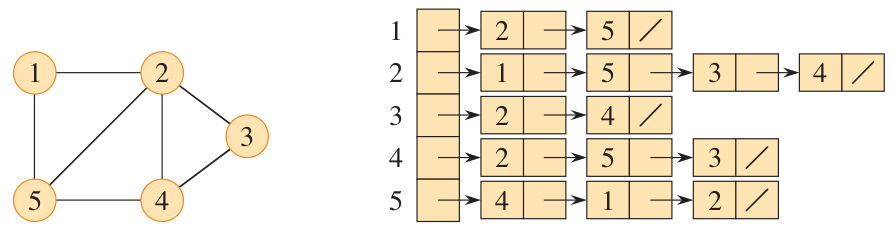
\includegraphics[width=0.6\textwidth]{figs/chap07/550-graph1-adj}
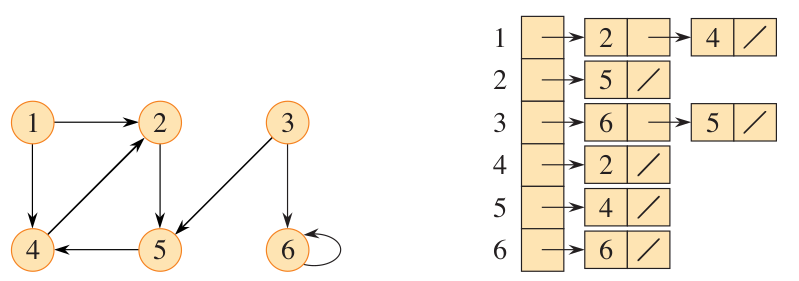
\includegraphics[width=0.6\textwidth]{figs/chap07/550-graph2-adj}
\end{figure}
\end{itemize}
\end{frame}


\begin{frame}{‌الگوریتم‌های گراف}
\begin{itemize}\itemr
\item[-]
اگر
\m{G}
یک گراف جهت‌دار باشد، مجموع اندازه همهٔ لیست‌های مجاورت برابراست با
\m{|E|}
، زیرا هریک از یال‌های
\m{(u,v)}
توسط درایهٔ
\m{Adj[u]}
نشان داده می‌شود.
\item[-]
اگر
\m{G}
یک گراف بدون جهت باشد، آنگاه مجموع اندازهٔ همهٔ لیست‌های مجاورت برابراست با
\m{2|E|}
، زیرا هر یک از یال‌های
\m{(u,v)}
هم در
\m{Adj[u]}
و هم در
\m{Adj[v]}
نمایش داده می‌شود.
\item[-]
فضای حافظه‌ای که لیست مجاورت برای نگهداری گراف نیاز دارد برابراست با
\ath{V+E} .
\iffalse
یافتن یک یال در گراف نیز به زمان
\ath{V+E}
نیاز دارد، زیرا برای یافتن یک یال همهٔ
\m{|V|}
درایهٔ لیست مجاورت باید بررسی شوند.
\fi
\end{itemize}
\end{frame}


\begin{frame}{‌الگوریتم‌های گراف}
\begin{itemize}\itemr
\item[-]
توسط لیست مجاورت می‌توانیم گراف‌های وزن‌دار
\fn{1}{weighted graphs}
را نیز نمایش دهیم.
در یک گراف وزن‌دار، هریک از یال‌ها دارای یک وزن است که توسط تابع وزن
\fn{2}{weight function}
\m{w : E \rightarrow \RR}
تولید می‌شود.
\item[-]
برای مثال فرض کنید
\m{G = (V,E)}
یک گراف وزن‌دار با تابع وزن
\m{w}
باشد. آنگاه می‌توانیم وزن
\m{w(u,v)}
از یال
\m{(u,v) \in E}
را در کنار رأس
\m{v}
در لیست مجاورت
\m{u}
ذخیره کنیم و نمایش دهیم.
\item[-]
یکی از معایب لیست مجاورت این است که برای پیدا کردن یال
\m{(u,v)}
سریع‌ترین روش ممکن جستجوی
\m{v}
در لیست مجاورت
\m{Adj[u]}
است.
\item[-]
ماتریس مجاورت برای پیدا کردن یک یال می‌تواند از لیست مجاورت سریع‌تر عمل کند.
\end{itemize}
\end{frame}


\begin{frame}{‌الگوریتم‌های گراف}
\begin{itemize}\itemr
\item[-]
در نمایش ماتریس مجاورت
\fn{1}{adjacency matrix representation}
برای گراف
\m{G = (V,E)}
فرض می‌کنیم هر رأس یک شماره از 
\m{1}
 تا
\m{|V|}
داشته باشد. سپس گراف
\m{G}
را با استفاده از ماتریس
\m{A = (a_{ij})}
با اندازهٔ
\m{|V| \times |V|}
نشان می‌دهیم به طوری‌که
\begin{align*}
\m{a_{ij}}  = \left\{ \begin{array}{lr}
				\m{1} & \m{(i,j) \in E}~\text{اگر}\\
					\m{0} & \text{در غیر اینصورت}
					\end{array}\right.
\end{align*}
\end{itemize}
\end{frame}


\begin{frame}{‌الگوریتم‌های گراف}
\begin{itemize}\itemr
\item[-]
در شکل زیر دو ماتریس مجاورت نشان داده شده‌اند.
\begin{figure}
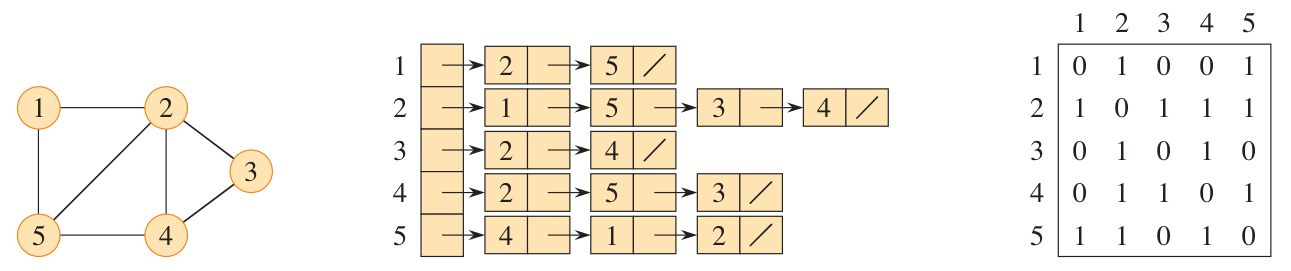
\includegraphics[width=0.9\textwidth]{figs/chap07/550-graph1}
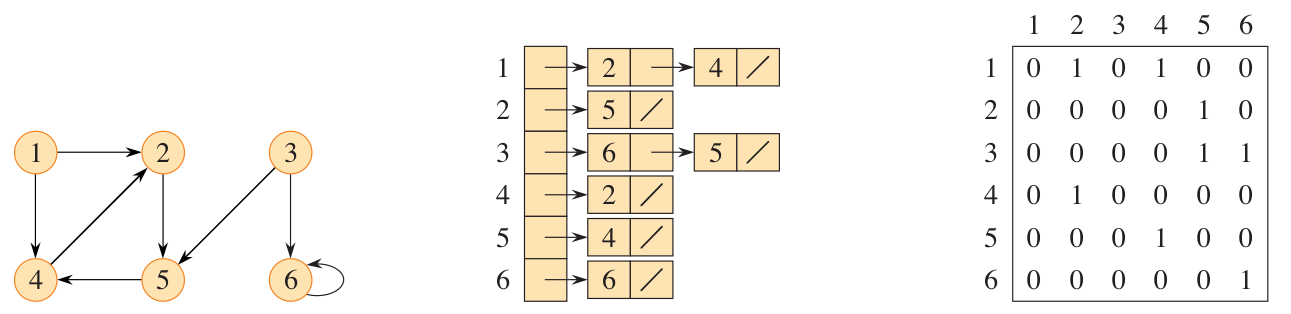
\includegraphics[width=0.9\textwidth]{figs/chap07/550-graph2}
\end{figure}
\end{itemize}
\end{frame}


\begin{frame}{‌الگوریتم‌های گراف}
\begin{itemize}\itemr
\item[-]
ماتریس مجاورت به حافظه
\ath{V^2}
برای نگهداری گراف نیاز دارد. برای یافتن یال
\m{(u,v)}
در گراف می‌توانیم درایهٔ
\m{A[u,v]}
را بررسی کنیم و بنابراین یافتن یک یال در گراف در زمان
\ath{1}
انجام می‌شود.
\item[-]
برای یک گراف بدون جهت، گراف نسبت به قطر اصلی‌اش متقارن است، زیرا
\m{A[u,v]}
برابراست با
\m{A[v,u]}
بنابراین ماتریس مجاورت برابر با ترانهادهٔ
\fn{1}{transpose}
 آن است و داریم
\m{A = A^T} .
\item[-]
اما در یک گراف جهت‌دار می‌توانیم یالی از
\m{u}
به
\m{v}
داشته باشیم بدون اینکه یال از
\m{v}
به
\m{u}
وجود داشته باشد.
\end{itemize}
\end{frame}


\begin{frame}{‌الگوریتم‌های گراف}
\begin{itemize}\itemr
\item[-]
با استفاده از ماتریس مجاورت می‌توانیم یک گراف وزن‌دار را نیز نمایش دهیم.
\item[-]
برای مثال، اگر
\m{G = (V,E)}
یک گراف وزن‌دار با تابع وزن
\m{w}
باشد، می‌توان وزن
\m{w(u,v)}
برای یال
\m{(u,v) \in E}
را به عنوان درایهٔ ماتریس مجاورت در سطر
\m{u}
و ستون
\m{v}
ذخیره کرد.
\item[-]
استفاده از ماتریس مجاورت در عمل راحت‌تر است اما به ازای گراف‌های بزرگ خلوت ممکن است فضای حافظه مورد نیاز آنها بسیار زیاد شود.
برای ذخیره‌سازی گراف‌های خلوت جهت‌دار، لیست مجاورت نسبت به ماتریس مجاورت فضای بسیار کمتری اشغال می‌کند.
\end{itemize}
\end{frame}

\begin{frame}{‌جستجوی سطح‌اول}
\begin{itemize}\itemr
\item[-]
جستجوی سطح‌اول
\fn{1}{breadth-first search}
یکی از ساده‌ترین الگوریتم‌های جستجوی گراف است که در بسیاری از الگوریتم‌های گراف استفاده می‌شود. برای مثال الگوریتم دایکسترا برای یافتن کوتاهترین مسیر بین دو رأس از جستجوی سطح‌اول استفاده می‌کند.
\item[-]
به ازای گراف دلخواه
\m{G=(V,E)}
و یک رأس مبدأ
\fn{2}{source vertic}
به نام
\m{s}
، الگوریتم جستجوی سطح‌اول همهٔ یال‌های گراف
\m{G}
را با شروع از رأس
\m{s}
بررسی می‌کند.
\item[-]
با شروع از رأس
\m{s}
، الگوریتم سطح‌اول ابتدا رئوسی را بررسی می‌کند که به
\m{s}
نزدیک‌ترند،
بدین معنی که برای رسیدن به آن رئوس از
\m{s}
باید از تعداد یال‌های کمتری عبور کرد.
\end{itemize}
\end{frame}


\begin{frame}{‌جستجوی سطح‌اول}
\begin{itemize}\itemr
\item[-]
یال‌هایی که در جستجوی سطح‌اول به ترتیب بررسی می‌شوند، یک درخت سطح‌اول می‌سازد که ریشهٔ آن
\m{s}
است و به ازای هر یک از رئوس
\m{v}
، یک مسیر ساده از
\m{s}
به
\m{v}
کوتاهترین مسیر از
\m{s}
به
\m{v}
در گراف را نشان می‌دهد.
در اینجا کوتاهترین مسیر درواقع مسیری است که دارای کمترین تعداد یال باشد.
\item[-]
جستجوی سطح‌اول، بدین دلیل سطح‌اول نامیده می‌شود که به ازای هر رأس
\m{v}
ابتدا رئوس مجاور آن بررسی  می‌شوند، قبل از اینکه رئوس مجاور مجاور آن بررسی شوند.
بنابراین اگر نزدیکترین رئوس به یک رأس را در سطح در نظر بگیریم و دورترین رئوس را در عمق، جستجوی سطح‌اول، قبل از بررسی رئوس در عمق، همهٔ رئوس در سطح را بررسی می‌کند.
بنابراین برخلاف جستجوی عمق اول که به ازای هر رأس
\m{v}
یک رأس مجاور مجاور
\m{v}
 ممکن است قبل از یک رأس مجاور
\m{v}
  پیمایش شود، در جستجوی سطح‌اول همهٔ رئوس مجاور
\m{v}
قبل از پیمایش رئوس مجاور مجاور 
\m{v}
پیمایش می‌شوند.
\end{itemize}
\end{frame}


\begin{frame}{‌جستجوی سطح‌اول}
\begin{itemize}\itemr
\item[-]
 در جستجوی سطح‌اول با شروع از رأس
\m{s}
ابتدا رئوس مجاور
\fn{1}{adjacent}
 یا همسایه‌هایی
\fn{2}{neighbour}
  بررسی می‌شوند که فاصلهٔ آنها از
\m{s}
برابر ۱ است، سپس همسایه‌ها با فاصلهٔ ۲ بررسی می‌شوند، پس از آن همسایه‌ها با فاصلهٔ ۳ و به همین ترتیب الی آخر، تا وقتی که همه رئوس بررسی شده باشند.
\item[-]
در جستجوی سطح‌اول از یک صف استفاده می‌شود که در آن ابتدا همسایه‌ها با فاصله ۱، سپس همسایه‌ها با فاصلهٔ ۲ و به همین ترتیب الی آخر در صف قرار می‌گیرند. بنابراین با خارج کردن همسایه‌ها از صف به ترتیب فاصله، گراف به صورت سطح‌اول بررسی می‌شود.
\end{itemize}
\end{frame}


\begin{frame}{‌جستجوی سطح‌اول}
\begin{itemize}\itemr
\item[-]
در الگوریتم جستجوی سطح‌اول می‌توانیم برای هر رأس ۳ رنگ در نظر بگیریم : سفید، خاکستری و سیاه. همهٔ رئوس در ابتدا به رنگ سفید هستند و رئوسی که هیچ مسیری از
\m{s}
به آنها وجود ندارد تا انتها به رنگ سفید باقی می‌‌مانند. وقتی یک رأس برای اولین بار با شروع از
\m{s}
پیمایش می‌شود، آن رأس به رنگ خاکستری تبدیل می‌شود. رنگ خاکستری بدین معنی است که آن رأس در مرز جستجو قرار گرفته است. مرز جستجو در واقع مرز میان رئوس پیمایش نشده و رئوس پیمایش شده است. صفی که در جستجوی سطح‌اول استفاده می‌شود، شامل همهٔ رئوس خاکستری است.
\item[-]
رئوس خاکستری به ترتیب از صف خارج می‌شوند و به رنگ سیاه تبدیل می‌شوند و رئوس سفید همسایهٔ آنها که تاکنون پیمایش نشده‌اند به رنگ خاکستری تبدیل می‌شوند و وارد صف می‌شوند.
\end{itemize}
\end{frame}


\begin{frame}{‌جستجوی سطح‌اول}
\begin{itemize}\itemr
\item[-]
یک الگوریتم جستجوی سطح‌اول، یک درخت سطح‌اول می‌سازد که ریشهٔ آن رأس
\m{s}
است. هرگاه در فرایند جستجو، یک رأس سفید
\m{v}
که در لیست همسایه‌های رأس خاکستری
\m{u}
 قرار دارد پیدا می‌شود، رأس
\m{v}
و یال
\m{(u,v)}
به درخت اضافه می‌شوند. می‌گوییم رأس
\m{u}
، سَلَف
\fn{1}{predecessor}
یا پدر رأس
\m{v}
و رأس
\m{v}
خَلَف
\fn{2}{successor}
یا فرزند رأس
\m{u}
در درخت سطح‌اول است. از آنجایی که هر رأس قابل دسترس از طریق
\m{s}
تنها یک بار بررسی می‌شود، هر رأس تنها یک پدر دارد.
\item[-]
تنها رأس ریشه، یعنی رأس
\m{s}
  دارای پدر نیست.
\item[-]
اگر رأس
\m{u}
بر روی یک مسیر ساده درخت از ریشه
\m{s}
به رأس
\m{v}
قرار بگیرد، آنگاه رأس
\m{u}
جد
\fn{3}{ancestor}
رأس
\m{v}
است و رأس
\m{v}
نوادهٔ
\fn{4}{descendant}
رأس
\m{u}
است.
\end{itemize}
\end{frame}


\begin{frame}{‌جستجوی سطح‌اول}
\begin{itemize}\itemr
\item[-]
در الگوریتم جستجوی سطح‌اول که بررسی خواهیم کرد،
\code{v.color}
رنگ رأس
\m{v}
است که می‌تواند سفید، خاکستری یا سیاه باشد،
\code{v.d}
فاصلهٔ رأس
\m{v}
از رأس
\m{s}
است و
\code{v.pred}
پدر رأس
\m{v}
است.
\item[-]
 رأس
\code{v.pred}
پدر
\fn{1}{predecessor}
 رأس
\code{v}
است، و رأس
\code{v}
فرزند
\fn{2}{successor}
رأس
\code{v.pred}
.
\end{itemize}
\end{frame}


\begin{frame}{‌جستجوی سطح‌اول}
\begin{itemize}\itemr
\item[-]
الگوریتم زیر جستجوی سطح‌اول را نشان می‌دهد.
\begin{algorithm}[H]\alglr
  \caption{Breadth-First Search} 
  \begin{algorithmic}[1]
   \Func{BFS}{G,s}
   \For{each vertex u $\in$ G.V - \{s\} }
   			\State u.color = White
   			\State u.d = $\infty$
   			\State u.pred = Nil
   	\EndFor
   	\State s.color = Gray
   	\State s.d = 0
   	\State s.pred = Nil
   	\State Q = $\emptyset$
   	\State Enqueue(Q,s)         
  \end{algorithmic}
  \label{alg:merge}
\end{algorithm}
\end{itemize}
\end{frame}


\begin{frame}{‌جستجوی سطح‌اول}
\begin{algorithm}[H]\alglr
  \caption{Breadth-First Search} 
  \begin{algorithmic}[1]
  \setcounter{ALG@line}{9}
   %\Func{Bfs}{G,s}			%\LeftComment{}
        \While{!empty(Q)}
        		\State u = Dequeue(Q)
        		\For{each vertex v in G.Adj[u]}		\LeftComment{search the neighbors of u}
        			\If{v.color == White}		\LeftComment{is v being discovered now?}
        				\State v.color = Gray
        				\State v.d = u.d + 1
        				\State v.pred = u
        				\State Enqueue(Q,v)		\LeftComment{v is now on the frontier}
        			\EndIf
        		\EndFor
        		\State u.color = Black		\LeftComment{u is now behind the frontier}
        \EndWhile		                   
  \end{algorithmic}
  \label{alg:merge}
\end{algorithm}
\end{frame}


\begin{frame}{‌جستجوی سطح‌اول}
\begin{itemize}\itemr
\item[-]
در شکل زیر یک گراف به صورت سطح‌اول پیمایش شده است.
\begin{figure}
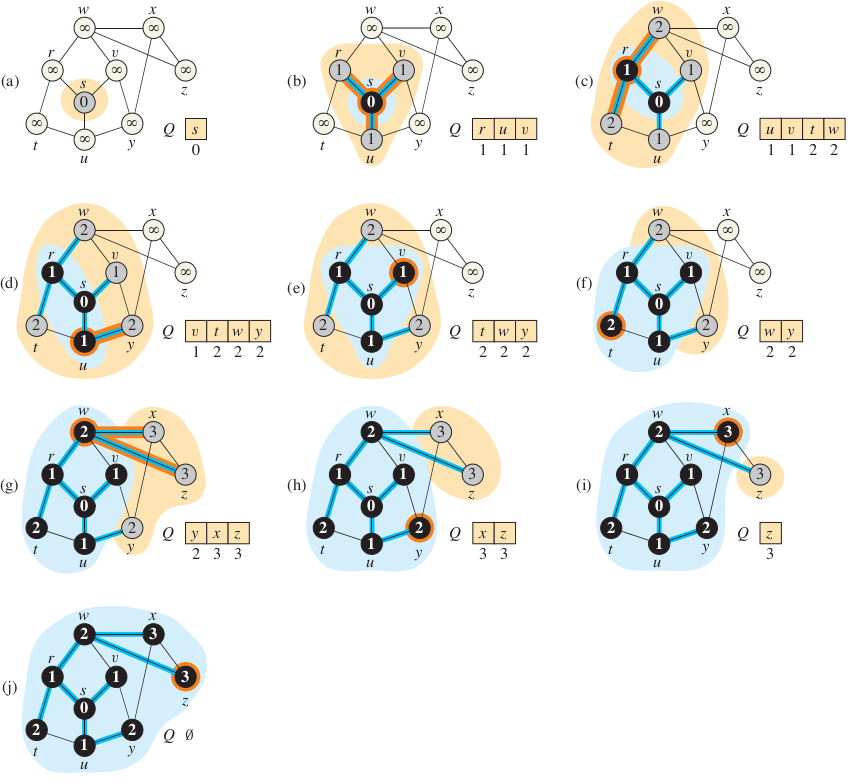
\includegraphics[width=0.5\textwidth]{figs/chap07/557-bfs}
\end{figure}
\end{itemize}
\end{frame}


\begin{frame}{‌جستجوی سطح‌اول}
\begin{itemize}\itemr
\item[-]
تحلیل الگوریتم جستجوی سطح‌اول : برای تحلیل الگوریتم جستجوی سطح‌اول می‌توانیم از تحلیل تجمعی استفاده کنیم. در این الگوریتم هیچ‌گاه یک رأس از رنگ خاکستری یا سیاه به رنگ سفید در نمی‌آید. هر رأس حداکثر یک بار وارد صف می‌شود و بنابراین هر رأس حداکثر یک بار از صف خارج می‌شود. عملیات اضافه کردن و برداشتن از صف در زمان
\m{O(1)}
انجام می‌شود.
خارج کردن رئوس از صف در زمان
\m{O(V)}
انجام می‌گیرد.
همچنین بررسی لیست مجاورت هر رأس حداکثر یک‌بار انجام می‌شود و مجموع طول همهٔ لیست‌های مجاورت برابر است با
\ath{E}
، بنابراین زمان لازم برای اجرای الگوریتم برابراست با
\m{O(V+E)}~.
نتیجه می‌گیریم جستجوی سطح‌اول در زمان خطی نسبت به اندازه لیست مجاورت اجرا می‌شود.
\item[-]
می‌توان ثابت کرد الگوریتم جستجوی سطح‌اول کوتاهترین مسیر از
\m{s}
به هریک از رئوس را محاسبه می‌کند.
\end{itemize}
\end{frame}

\iffalse
\begin{frame}{‌جستجوی سطح‌اول}
\begin{itemize}\itemr
\item[-]
حال می‌خواهیم اثبات کنیم الگوریتم جستجوی سطح‌اول کوتاهترین مسیر از رأس مبدأ
\m{s}
به هریک از رئوس گراف را پیدا می‌کند. فاصله کوتاهترین مسیر
\fn{1}{shortest path distance}
\m{\delta(s,v)}
از رأس
\m{s}
به
\m{v}
کمترین تعداد یال‌هایی است که در یک مسیر از
\m{s}
به
\m{v}
می‌توان پیمود. اگر هیچ مسیری از
\m{s}
به
\m{v}
وجود نداشته باشد، آنگاه
\m{\delta(s,v) = \infty}
مسیری که طول آن
\m{\delta(s,v)}
باشد کوتاهترین مسیر
\fn{2}{shortest path}
از
\m{s}
به
\m{v}
است.
\end{itemize}
\end{frame}
\fi

\begin{frame}{‌جستجوی عمق‌اول}
\begin{itemize}\itemr
\item[-]
جستجوی عمق‌اول به جای اینکه جستجو را در سطح شروع کند و همهٔ رئوس مجاور را در ابتدا پیمایش کند، به ازای هر رأس پیمایش شده، مجاور رأس را پیمایش می‌کند و به عبارت دیگر جستجو در عمق انجام می‌دهد.
\item[-]
برای روشن‌تر شدن جستجوی سطحی و عمقی مثال زیر را در نظر بگیرید. می‌خواهیم مطلبی را درون چندین کتاب جستجو کنیم. در یک جستجوی سطحی ابتدا به سراغ صفحه اول همهٔ کتاب‌ها می‌رویم تا این که در نهایت همهٔ کتاب‌ها را بررسی کنیم. در یک جستجوی عمقی ابتدا کتاب اول را تا انتها مطالعه می‌کنیم و در صورتی که مطلب مورد نظر را پیدا نکردیم به سراغ کتاب دوم می‌رویم تا این که در نهایت همهٔ کتاب‌ها را جستجو کنیم. در این مثال هیچ یک از جستجوها مزیتی بر دیگری ندارد چرا که مطلب مورد نظر ممکن است در صفحهٔ آخر کتاب اول باشد که در این صورت جستجوی عمقی زودتر به جواب می‌رسد و یا ممکن است مطلب مورد نظر در صفحه اول کتاب آخر باشد که در این صورت جستجوی سطح اول زودتر به جواب می‌رسد.
\end{itemize}
\end{frame}


\begin{frame}{‌جستجوی عمق‌اول}
\begin{itemize}\itemr
\item[-]
جستجوی عمق‌اول یال‌های بررسی نشدهٔ رئوس تازه پیدا شده را زودتر از یال‌های بررسی نشدهٔ رئوس قبلاً پیدا شده بررسی می‌کند. وقتی فرایند جستجو به نقطه‌ای رسید که یال‌های یک رأس همگی بررسی شده بودند، الگوریتم پسگرد می‌کند تا به رئوسی برسد که یال‌های آنها هنوز بررسی نشده‌اند.
\item[-]
در صورتی که یک رأس با شروع از رأس آغازین قابل دسترس نباشد، گراف همبند نیست و برای جستجوی کامل گراف، الگوریتم یکی از رئوس را به عنوان مبدأ جدید انتخاب کرده و جستجو را از رأس جدید آغاز می‌‌کند.
\end{itemize}
\end{frame}


\begin{frame}{‌جستجوی عمق‌اول}
\begin{itemize}\itemr
\item[-]
همانند جستجوی سطح اول، در جستجوی عمق‌اول توسط رنگ رأس‌ها وضعیت آنها مشخص می‌شود. هر رأس در ابتدا سفید است، هنگامی که برای اولین بار پیدا می‌شود به رنگ خاکستری تبدیل می‌شود و در پایان هنگامی که بررسی شد (بدین معنی که همهٔ رئوس در لیست مجاورت آن پیدا شدند) به رنگ سیاه در می‌آید.
\end{itemize}
\end{frame}


\begin{frame}{‌جستجوی عمق‌اول}
\begin{itemize}\itemr
\item[-]
در جستجوی عمق‌اول هر رأس دارای دو برچسب زمان
\fn{1}{time stamp}
است. برچسب زمان اول
\m{v.s}
زمانی نشان می‌دهد که رأس برای بار اول پیدا شده است و به رنگ خاکستری درآمده است و برچسب دوم
\m{v.f}
مشخص می‌کند که رأس
\m{v}
به طور کامل بررسی شده است بدین معنی که همهٔ رئوس لیست مجاورت آن پیدا شده‌اند و رأس
\m{v}
به رنگ مشکی درآمده است.
\end{itemize}
\end{frame}


\begin{frame}{‌جستجوی عمق‌اول}
\begin{itemize}\itemr
\item[-]
الگوریتم زیر جستجوی عمق‌اول را نشان می‌دهد.
\begin{algorithm}[H]\alglr
  \caption{Depth-First Search} 
  \begin{algorithmic}[1]
   \Func{DFS}{G}
   \For{each vertex u $\in$ G.V}
   			\State u.color = White
   			\State u.pred = Nil
   	\EndFor
   	\State time = 0
   	\For{each vertex u $\in$ G.V}
   			\If{u.color == White}
   					\State DFS-Visit(G,u)
   			\EndIf
   	\EndFor                           
  \end{algorithmic}
  \label{alg:merge}
\end{algorithm}
\end{itemize}
\end{frame}


\begin{frame}{‌جستجوی عمق‌اول}
\begin{itemize}\itemr
\item[-]
\begin{algorithm}[H]\alglr
  \caption{DFS-Visit} 
  \begin{algorithmic}[1]
   \Func{DFS-Visit}{G,u}
   \State time = time + 1		\LeftComment{white vertex u has just been discovered}
   \State u.s = time
   \State u.color = Gray
   \For{each vertex v in G.Adj[u]}		\LeftComment{explore each edge(u,v)}
   		\If{v.color == White}
   				\State v.pred = u
   				\State DFS-Visit(G,v)
   		\EndIf
   \EndFor
   \State time = time + 1
   \State u.f = time
   \State u.color = Black   \LeftComment{blacken u; it is finished}                           
  \end{algorithmic}
  \label{alg:merge}
\end{algorithm}
\end{itemize}
\end{frame}


\begin{frame}{‌جستجوی عمق‌اول}
\begin{itemize}\itemr
\item[-]
وقتی الگوریتم جستجوی عمق‌اول به اتمام می‌رسد هر رأس دارای دو برچسب زمان است که یکی زمان پیدا شدن
\fn{1}{discovery time}
و دیگری زمان به پایان رسیدن
\fn{2}{finish time}
را نشان می‌دهد.
\end{itemize}
\end{frame}


\begin{frame}{‌جستجوی عمق‌اول}
\begin{itemize}\itemr
\item[-]
در مثال زیر، گراف توسط الگوریتم عمق‌اول بررسی شده است.
\begin{figure}
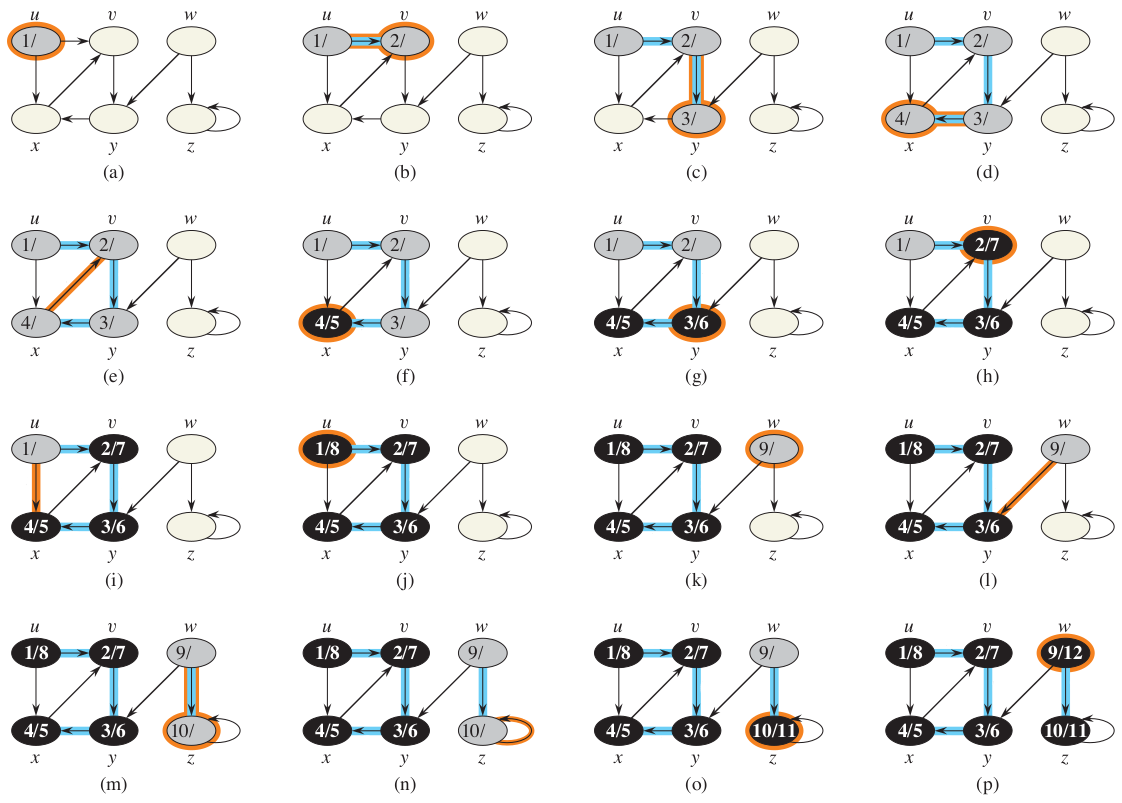
\includegraphics[width=0.6\textwidth]{figs/chap07/566-dfs}
\end{figure}
\end{itemize}
\end{frame}


\begin{frame}{‌جستجوی عمق‌اول}
\begin{itemize}\itemr
%\item[-]
%خطوط ۱ تا ۳ و خطوط ۵ تا ۷ در الگوریتم جستجوی عمق‌اول در زمان
%\ath{V}
%انجام می‌شوند.
\item[-]
در اینجا نیز برای تحلیل الگوریتم از تحلیل تجمعی استفاده می‌کنیم.
\item[-]
الگوریتم
\code{DFS-Visit}
برای هر رأس
\m{v \in V}
تنها یک بار فراخوانی می‌شود، چرا که این الگوریتم برای رئوس سفید فراخوانی می‌شود و آنها را به رنگ خاکستری تبدیل می‌کند. الگوریتم
\code{DFS-Visit}
به ازای هر رأس
\m{v}
در یک حلقه تکرار
\m{|Adj[v]|}
بار تکرار می‌شود. بنابراین برای همهٔ رئوس، این حلقه
\m{\sum_{v \in V} |Adj[v]| = \ath{E}}
بار تکرار می‌شود.
\item[-]
پس زمان اجرای الگوریتم جستجوی عمق‌اول
\ath{V+E}
است.
\end{itemize}
\end{frame}


\begin{frame}{‌جستجوی عمق‌اول}
\begin{itemize}\itemr
\item[-]
می‌توان اثبات کرد که در جستجوی عمق‌اول زمان پیدا شدن و زمان به اتمام رسیدن رئوس گراف یک ساختار پرانتز گذاری کامل دارند. اگر به ازای یافته شدن رأس
\m{u}
یک پرانتز به صورت
\m{"(u"}
باز کنیم و به ازای به اتمام رسیدن بررسی رأس
\m{u}
پرانتز را به صورت
\m{"u)"}
ببندیم، یک عبارت با پرانتزگذاری کامل به دست می‌آید بدین معنی که پرانتزها تودرتو هستند.
\end{itemize}
\end{frame}


\begin{frame}{‌جستجوی عمق‌اول}
\begin{itemize}\itemr
\item[-]
از جستجوی عمق‌اول در مرتب‌سازی توپولوژیکی
\fn{1}{topological sort}
یا مرتب‌سازی موضعی
یک گراف بدون دور
\fn{2}{acyclic graph}
استفاده می‌شود.
\item[-]
یک مرتب‌سازی توپولوژیکی در یک گراف بدون دور
\m{G=(V,E)}
رئوس گراف را به گونه‌ای مرتب می‌کند که اگر
\m{G}
شامل یال
\m{(u,v)}
باشد، آنگاه
\m{u}
قبل از
\m{v}
در آرایهٔ مرتب شده قرار می‌گیرد.
\item[-]
مرتب‌سازی توپولوژیکی تنها برای گراف‌های جهت‌دار بدون دور
\fn{3}{directed acyclic graph}
تعریف می‌شود.
\item[-]
مرتب‌سازی توپولوژیکی به گونه‌ای است که اگر رئوس مرتب شده برروی یک خط افقی قرار بگیرند، جهت همهٔ یال‌های از چپ به راست است.
\end{itemize}
\end{frame}


\begin{frame}{‌جستجوی عمق‌اول}
\begin{itemize}\itemr
\item[-]
از یک گراف جهت‌دار بدون دور می‌توان برای نمایش دادن رویداد‌ها
\fn{1}{event}
استفاده کرد.
\item[-]
برای مثال در شکل زیر برای یک گراف شامل تعدادی رویداد مرتب‌سازی توپولوژیکی انجام شده است.
\begin{figure}
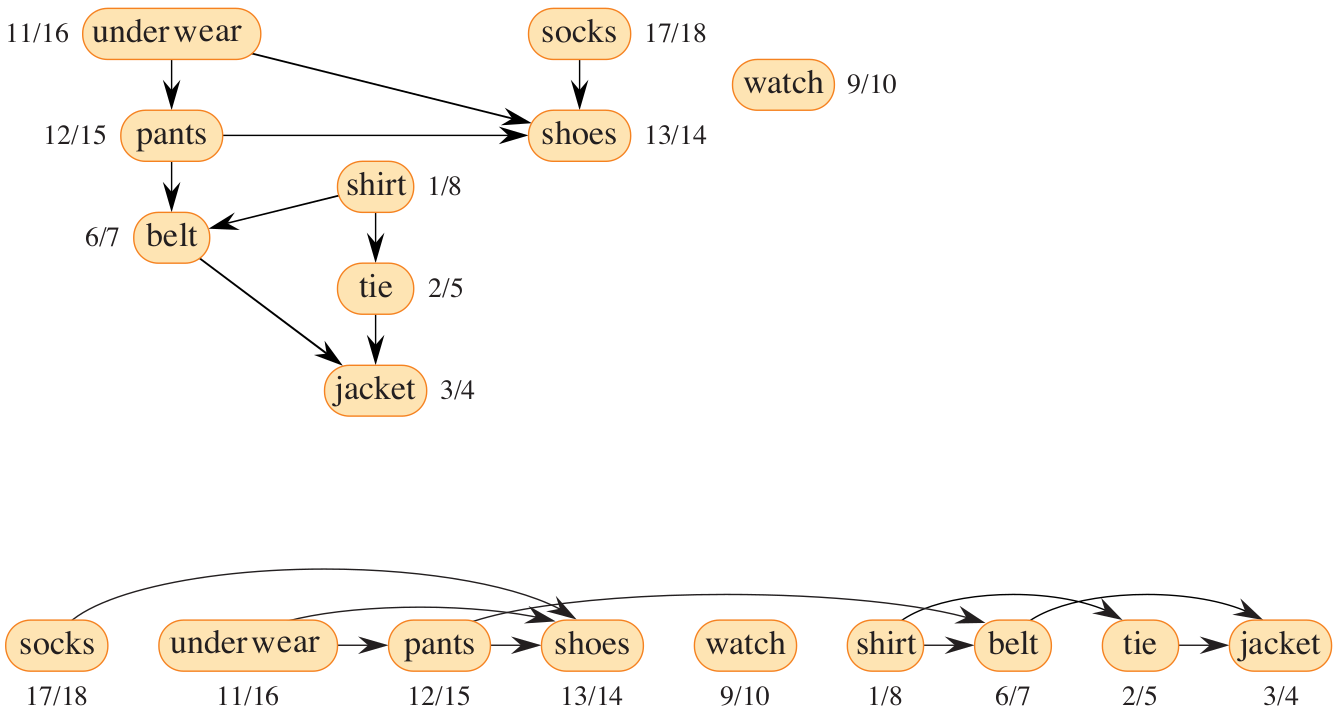
\includegraphics[width=0.6\textwidth]{figs/chap07/574-topological}
\end{figure}
\end{itemize}
\end{frame}

\begin{frame}{‌درخت پوشای کمینه}
\begin{itemize}\itemr
\item[-]
در طراحی مدارهای الکتریکی، معمولاً طراحان نیاز دارند که قسمت‌هایی از مدار را که در یک سطح ولتاژ قرار دارند، به یکدیگر متصل کنند. برای متصل کردن
\m{n}
نقطه به یکدیگر، به
\m{n-1}
سیم نیاز داریم که به شکل‌های متفاوت می‌توانند هر یک  دو نقطه را به یکدیگر متصل کنند. در چنین مسئله‌ای هدف یافتن روشی برای اتصال است که در آن از کمترین مقدار سیم لازم استفاده می‌کنیم. برای مدلسازی این مسئله به صورت زیر عمل می‌کنیم.
\item[-]
گراف
\m{G = (V,E)}
را با وزن‌های
\m{w : E \to \RR}
در نظر بگیرید. وزن یال
\m{(u,v) \in E}
برابر است با
\m{w(u,v)} .
\end{itemize}
\end{frame}


\begin{frame}{‌درخت پوشای کمینه}
\begin{itemize}\itemr
\item[-]
نقطه‌ها در یک مدار الکتریکی معادل رئوس گراف و سیم‌ها معادل یال‌های گراف هستند. مقدار سیمی که برای اتصال یک نقطه به نقطه دیگر نیاز است را با وزن یال مدلسازی می‌کنیم.
\item[-]
هدف پیدا کردن زیر مجموعهٔ
\m{ T \subseteq E}
است که همهٔ رئوس گراف را به یکدیگر متصل می‌کند و وزن کل آن برابر با
\m{w(T) = \sum_{(u,v) \in T} w(u,v)}
کمینه است.
\item[-]
زیرمجموعهٔ
\m{ T }
همهٔ رأس‌های گراف را به یکدیگر متصل می‌کند و دارای هیچ دوری نیست، پس یک درخت را تشکیل می‌دهد. به چنین درختی، درخت پوشا
\fn{1}{spanning tree}
گفته می‌شود. مسئله درخت پوشای کمینه
\fn{2}{minimum spanning tree problem}
به دنبال درخت پوشایی می‌گردد که وزن آن از همهٔ درخت‌های پوشای دیگر کمتر باشد.
\end{itemize}
\end{frame}


\begin{frame}{‌درخت پوشای کمینه}
\begin{itemize}\itemr
\item[-]
ورودی مسئله درخت پوشای کمینه گراف همبند بدون جهت
\m{G = (V,E)}
است که تابع وزن یال‌های آن
\m{w : E \rightarrow \RR}
است. هدف یافتن یک درخت پوشای کمینه برای
\m{G}
است.
\item[-]
دو الگوریتم حریصانه برای یافتن درخت پوشای کمینه معرفی خواهیم کرد که روش آنها مشابه است ولی پیاده‌سازی آنها متفاوت است.
\item[-]
این استراتژی را به عنوان یک الگوریتم کلی برای یافتن درخت پوشای کمینه معرفی می‌کنیم.
\end{itemize}
\end{frame}


\begin{frame}{‌درخت پوشای کمینه}
\begin{itemize}\itemr
\item[-]
الگوریتم کلی برای یافتن درخت پوشای کمینه به صورت زیر است.
\begin{algorithm}[H]\alglr
  \caption{Generic-MST} 
  \begin{algorithmic}[1]
   \Func{Generic-MST}{G,w}
   \State A =$\emptyset$
   \While{A does not form a spanning tree}
   			\State find an edge (u,v) that is safe for A
   			\State A = A $\cup$ {(u,v)}
   	\EndWhile
   	\State \Return A               
  \end{algorithmic}
  \label{alg:merge}
\end{algorithm}
\end{itemize}
\end{frame}


\begin{frame}{‌درخت پوشای کمینه}
\begin{itemize}\itemr
\item[-]
قبل از هر تکرار در حلقه،
\m{A}
یک زیر مجموعه از یک درخت پوشای کمینه است.
\item[-]
در هر گام از الگوریتم، یال
\m{(u,v)}
به
\m{A}
اضافه می‌شود بدون اینکه ویژگی
\m{A}
تغییر کند. به عبارت دیگر
\m{A \cup {(u,v)}}
نیز زیرمجموعه‌ای از درخت پوشای کمینه است.
\item[-]
یالی که به
\m{A}
اضافه می‌شود را یک یال مطمئن
\fn{1}{safe edge}
می‌نامیم زیرا ویژگی درخت را حفظ می‌کند.
\item[-]
پس در گام اول قبل از شروع حلقه ویژگی درخت (که زیرمجموعهٔ درخت پوشای کمینه است) برقرار است. در هرگام در حلقه تکرار ویژگی درخت حفظ می‌شود، پس در پایان یک درخت پوشای کمینه خواهیم داشت.
\end{itemize}
\end{frame}


\begin{frame}{‌درخت پوشای کمینه}
\begin{itemize}\itemr
\item[-]
حال روشی برای یافتن یال مطمئن ارائه می‌‌دهیم.
\item[-]
قبل از بررسی ویژگی یال مطمئن چند تعریف ارائه می‌کنیم.
\item[-]
یک برش
\fn{1}{cut}
\m{(S,V-S)}
از یک گراف بدون جهت
\m{G = (V,E)}
یک تقسیم‌بندی از رئوس
\m{V}
است که در آن مجموعهٔ رئوس به دو قسمت تقسیم می‌شوند.
\item[-]
می‌گوییم یال
\m{(u,v) \in E}
از برش
\m{(S,V-S)}
عبور می‌کند
\fn{1}{crosses}
اگر یک رأس یال در مجموعهٔ
\m{S}
و رأس دیگر یال در مجموعهٔ
\m{V-S}
قرار بگیرد.
\item[-]
یالی را که از یک برش عبور می‌کند یال سبک
\fn{3}{light edge}
می‌نامیم اگر وزن آن در بین همهٔ یال‌هایی که از برش عبور می‌کنند کمینه باشد. در یک برش ممکن است چند یال سبک هم‌وزن وجود داشته باشند.
\end{itemize}
\end{frame}


\begin{frame}{‌درخت پوشای کمینه}
\begin{itemize}\itemr
\item[-]
شکل زیر یک برش را نشان می‌دهد.
یال سبک در این برش یال 
\m{(c, d)}
با وزن ۷ است.
\begin{figure}
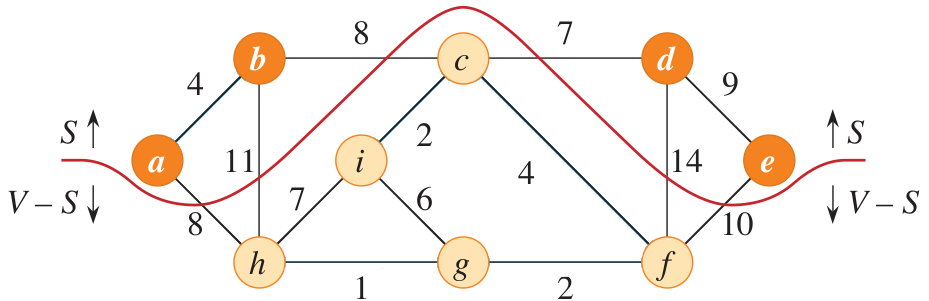
\includegraphics[width=0.9\textwidth]{figs/chap07/588-cut}
\end{figure}
\end{itemize}
\end{frame}


\begin{frame}{‌درخت پوشای کمینه}
\begin{itemize}\itemr
\item[-]
قضیه : فرض کنید
\m{G = (V,E)}
یک گراف همبند بدون جهت با یال‌های وزن‌دار باشد و وزن‌ها با تابع
\m{w}
تعریف شده باشند. فرض کنید
\m{A}
یک زیرمجموعه از
\m{E}
باشد که در یک درخت پوشای کمینه برای
\m{G}
قرار گرفته باشد و فرض کنید
\m{(S,V-S)}
یک برش از
\m{G}
باشد که هیچ یالی در
\m{A}
از آن
عبور نمی‌کند. فرض کنید
\m{(u,v)}
یک یال سبک باشد که از برش
\m{(S,V-S)}
عبور می‌کند. آنگاه یال
\m{(u,v)}
یک یال مطمئن برای
\m{A}
است.
\item[-]
اثبات:
از برهان خلف استفاده می‌کنیم.
فرض کنیم 
\m{(u,v)}
یک یال مطمئن برای 
\m{A}
نیست.
از آنجایی که 
درخت پوشای کمینه همبند است و در آن دور وجود ندارد، 
\m{u}
و
\m{v}
باید از طریق یک مسیر یکتا به یکدیگر متصل شده باشند.
حال یالی که 
\m{S}
و
\m{V-S}
را به یکدیگر متصل می‌کند از درخت پوشای کمینه حذف می‌کنیم و 
\m{(u,v)}
را جایگزین آن می‌کنیم. درخت پوشای به دست آمده هزینه‌اش از درخت قبلی بیشتر نیست و بنابراین کمینه است. پس یال
\m{(u,v)}
یک یال مطمئن است.
\end{itemize}
\end{frame}


\iffalse
\begin{frame}{‌درخت پوشای کمینه}
\begin{itemize}\itemr
\item[-]
اثبات : فرض کنید
\m{T}
یک درخت پوشای کمینه باشد که
\m{A}
را شامل می‌شود. درخت پوشای کمینه
\m{T'}
را به گونه‌ای می‌سازیم که شامل
\m{A \cup {(u,v)}}
شود و نشان می‌دهیم که
\m{(u,v)}
یک یال مطمئن برای
\m{A}
است.
\item[-]
از آنجایی که 
درخت پوشای کمینه همبند است و در آن دور وجود ندارد، 
\m{u}
و
\m{v}
باید از طریق یک مسیر یکتا به یکدیگر متصل شده باشند.
 مسیر ساده
\m{p}
از رأس
\m{u}
به
\m{v}
در درخت
\m{T}
را در نظر بگیرید.
\item[-]
شکل زیر این حالت را نشان می‌دهد.
\begin{figure}
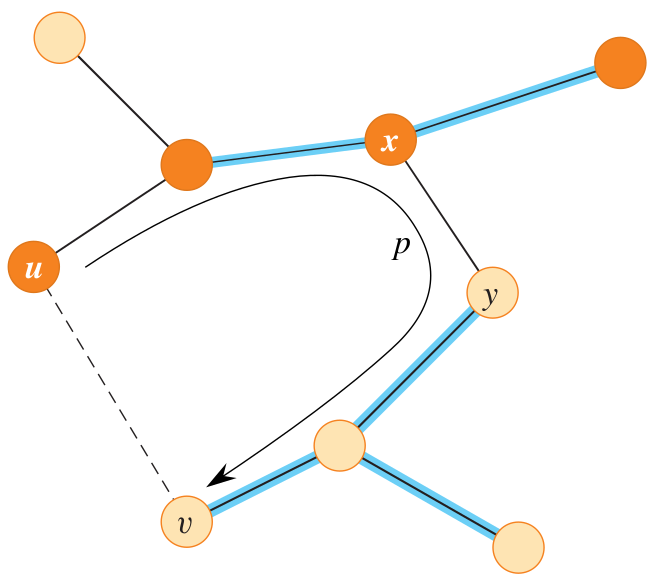
\includegraphics[width=0.3\textwidth]{figs/chap07/589-proof}
\end{figure}
\end{itemize}
\end{frame}


\begin{frame}{‌درخت پوشای کمینه}
\begin{itemize}\itemr
\item[-]
از آنجایی که
\m{u}
و
\m{v}
در دو طرف برش
\m{(S,V-S)}
قرار دارند، حداقل یک یال در
\m{T}
وجود دارد که بر روی مسیر سادهٔ
\m{p}
است و همچنین از برش عبور می‌کند. فرض کنید
\m{(x,y)}
چنین یالی باشد.
\item[-]
یال
\m{(x,y)}
در
\m{A}
نیست، زیرا می‌دانیم برش از یال‌های
\m{A}
عبور نمی‌کند.
\item[-]
از آنجایی که
\m{(x,y)}
یک مسیر ساده یکتا از
\m{u}
به
\m{v}
در
\m{T}
است، حذف کردن
\m{(x,y)}
درخت
\m{T}
را به دو جزء تقسیم می‌کند. اضافه کردن
\m{(u,v)}
آن دو جزء را دوباره به یکدیگر متصل می‌کند و درخت پوشای جدید
\m{T' = (T - \{(x,y)\}) \cup \{(u,v)\}}
را می‌سازد.
\end{itemize}
\end{frame}


\begin{frame}{‌درخت پوشای کمینه}
\begin{itemize}\itemr
\item[-]
حال نشان می‌دهیم
\m{T'}
یک درخت پوشای کمینه است. از آنجایی که
\m{(u,v)}
یک یال سبک است که از
\m{(S,V-S)}
عبور می‌کند و
\m{(x,y)}
نیز از این برش عبور می‌کند
\m{w(u,v) \leqslant w(x,y)}
. بنابراین :
\begin{align*}
\m{w(T') = w(T) - w(x,y) + w(u,v) \leqslant w(T)}
\end{align*}
\item[-]
اما
\m{T}
یک درخت پوشای کمینه است، بنابراین
\m{w(T) \leqslant w(T')}
و بنابراین
\m{T'}
باید یک درخت پوشای کمینه باشد.
\item[-]
حال باید نشان دهیم
\m{(u,v)}
یک یال سبک برای
\m{A}
است. داریم
\m{A \subseteq T'}
بنابراین
\m{A \subseteq T}
و
\m{(x,y) \notin A}
بنابراین
\m{A \cup{(u,v)} \subseteq T'}
بنابراین از آنجایی که
\m{T'}
یک درخت پوشای کمینه است،
\m{(u,v)}
برای
\m{A}
مطمئن است.
\end{itemize}
\end{frame}
\fi

\begin{frame}{‌الگوریتم پریم}
\begin{itemize}\itemr
\item[-]
الگوریتم پریم مطابق با قضیه‌ای که بیان شد طراحی شده است.
\item[-]
در الگوریتم پریم
\fn{1}{Prim's algorithm}
 یال‌های مجموعهٔ
\m{A}
(زیرمجموعهٔ یال‌های درخت پوشای کمینه)
همیشه یک درخت را تشکیل می‌دهند.
\item[-]
درخت پوشای کمینه با یک رأس ریشه
%\m{r}
آغاز می‌شود تا در نهایت همهٔ یال‌ها
%\m{V}
را پوشش دهد. در هرگام یک یال سبک به درخت
\m{A}
افزوده می‌شود که
\m{A}
را به یک رأس متصل می‌کند.
\item[-]
این الگوریتم یک الگوریتم حریصانه است، زیرا در هر مرحله یک یال با وزن کمینه به درخت افزوده می‌شود.
\end{itemize}
\end{frame}


\begin{frame}{‌الگوریتم پریم}
\begin{itemize}\itemr
\item[-]
شکل زیر روند اجرای الگوریتم پریم را نشان می‌دهد.
\begin{figure}
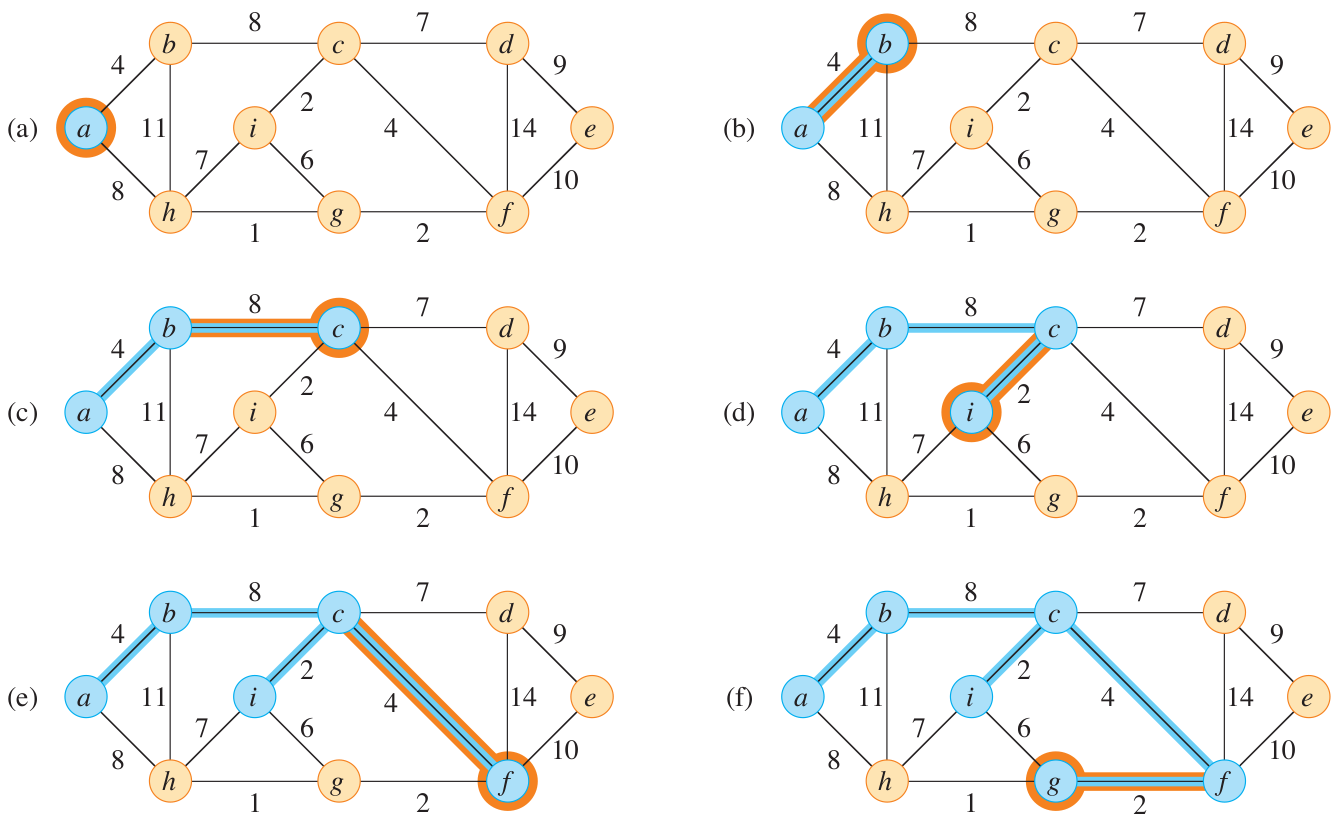
\includegraphics[width=0.6\textwidth]{figs/chap07/595-prim-1}
\end{figure}
\end{itemize}
\end{frame}

\begin{frame}{‌الگوریتم پریم}
\begin{itemize}\itemr
\item[-]
شکل زیر روند اجرای الگوریتم پریم را نشان می‌دهد.
\begin{figure}
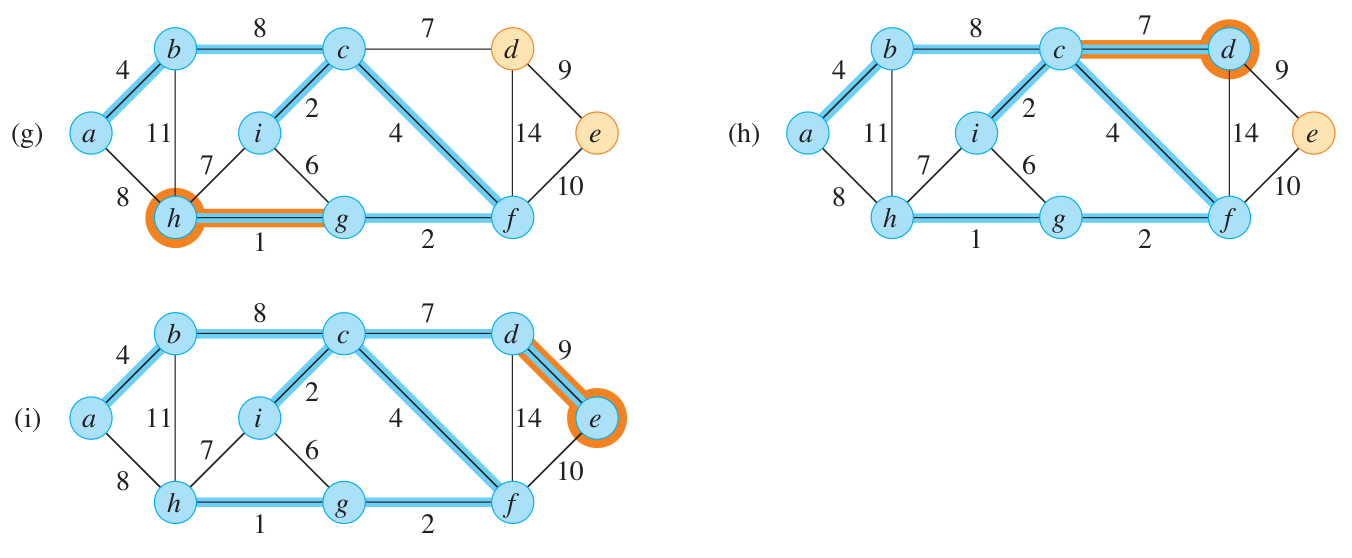
\includegraphics[width=0.6\textwidth]{figs/chap07/595-prim-2}
\end{figure}
\end{itemize}
\end{frame}

\begin{frame}{‌الگوریتم پریم}
\begin{itemize}\itemr
\item[-]
الگوریتم پریم در زیر نشان داده شده است.
\begin{algorithm}[H]\alglr
  \caption{Minimum Spanning Tree - Prim} 
  \begin{algorithmic}[1]
   \Func{Mst-Prim}{G,w,r}
   \For{each vertex u $\in$ G.V}
   		\State u.key = $\infty$
   		\State u.pred = Nil
   	\EndFor
   	\State r.key = 0
   	\State Q = $\emptyset$
   	\For{each vertex u $\in$ G.V}
   			\State Insert(Q,u)
   	\EndFor                    
  \end{algorithmic}
  \label{alg:merge}
\end{algorithm}
\end{itemize}
\end{frame}


\begin{frame}{‌الگوریتم پریم}
\begin{itemize}\itemr
\item[-]
\begin{algorithm}[H]\alglr
  \caption{Minimum Spanning Tree - Prim} 
  \begin{algorithmic}[1]
   \setcounter{ALG@line}{7}
   %\Func{Mst-Prim}{G,w,r}
   	\While{Q $\neq$ $\emptyset$}
   			\State u = Extract-Min(Q)		\LeftComment{add u to the tree}
   			\For{each vertex v in G.Adj[u]}		\LeftComment{update keys of u's non-tree neighbors}
   					\If{v $\in$ Q and w(u,v) < v.key}
   							\State v.pred = u
   							\State v.key = w(u,v)
   							\State Decrease-Key(Q,v,w(u,v))
   					\EndIf
   			\EndFor
   	\EndWhile                           
  \end{algorithmic}
  \label{alg:merge}
\end{algorithm}
\end{itemize}
\end{frame}


\begin{frame}{‌الگوریتم پریم}
\begin{itemize}\itemr
\item[-]
برای اضافه کردن یال جدید به درخت
\m{A}
، الگوریتم از صف اولویت
\m{Q}
استفاده می‌کند که در آن رئوسی که به درخت افزوده نشده‌اند نگهداری می‌شود.
\item[-]
برای هر رأس
\m{v}
، ویژگی
\m{v.key}
وزن کمینه یالی است که
\m{v}
را به یک رأس دیگر در درخت متصل می‌کند.
\item[-]
مقدار
\m{v.pred}
پدر رأس
\m{v}
را در درخت مشخص می‌کند.
\end{itemize}
\end{frame}


\iffalse
\begin{frame}{‌الگوریتم پریم}
\begin{itemize}\itemr
\item[-]
به طور ضمنی در این الگوریتم مجموعه
\m{A}
حاوی
\m{A = \{(v,v.pred) : v \in V-\{r\}-Q\}}
است.
\item[-]
وقتی الگوریتم به پایان می‌رسد، صف اولویت خالی می‌شود و در نتیجه داریم :
\begin{align*}
\m{A = \{(v,v.pred) : v \in V-\{r\}\}}
\end{align*}
\end{itemize}
\end{frame}
\fi



\begin{frame}{‌الگوریتم پریم}
\begin{itemize}\itemr
\item[-]
زمان اجرای الگوریتم پریم را به صورت زیر تحلیل می‌کنیم.
%به نحوه پیاده‌سازی صف اولویت بستگی دارد.
\item[-]
حلقهٔ
\code{while}
به تعداد
\m{|V|}
بار تکرار می‌شود و از آنجایی که عملیات
\code{Extract-Min}
در زمان
\m{O(lg|V|)}
اجرا می‌شود، زمان لازم برای انجام این عملیات
\m{O(|V|lg|V|)}
است.
\item[-]
حلقهٔ
\code{for}
در خطوط ۱۰ تا ۱۴ جمعاً
\m{O(|E|)}
بار تکرار می‌شود. هر فراخوانی
\code{Decrease-Key}
در زمان
\m{O(lg|V|)}
اجرا می‌شود، بنابراین الگوریتم پریم در زمان
\m{O(|V|lg|V|+|E|lg|V|)}
اجرا می‌شود. چون تعداد یال‌های گرافی که دارای درخت پوشای کمینه است، حداقل برابر با 
\m{|V|}
است، پس زمان اجرای الگوریتم پریم برابر با
\m{O(|E|lg|V|)}
 است.
\end{itemize}
\end{frame}

\iffalse
\begin{frame}{‌الگوریتم پریم}
\begin{itemize}\itemr
\item[-]
اگر صف اولویت با یک هرم فیبوناچی
\fn{1}{Fibonacci heap}
پیاده‌سازی شود، زمان اجرای الگوریتم پریم بهبود می‌یابد.
\item[-]
اگر هرم فیبوناچی تعداد
\m{|V|}
عنصر را نگهداری کند، تابع
\code{Exract-Min}
در زمان
\m{O(lgV)}
اجرا می‌شود و هریک از عملیات
\code{Insert}
و
\code{Decrease-Key}
در
\m{O(1)}
اجرا می‌شوند. بنابراین الگوریتم پریم می‌تواند در زمان
\m{O(E+VlgV)}
اجرا شود.
\end{itemize}
\end{frame}
\fi

\begin{frame}{‌الگوریتم کروسکال}
\begin{itemize}\itemr
\item[-]
الگوریتم کروسکال ابتدا به ازای هر رأس یک مجموعهٔ مجزا ایجاد می‌کند. سپس برای یافتن یال مطمئن در هر مرحله از بین همهٔ یال‌هایی که دو رأس در دو مجموعهٔ مجزا را به یکدیگر متصل می‌کنند، یال
\m{(u,v)}
با کمترین وزن را انتخاب می‌کند.
وقتی یال
\m{(u,v)}
به عنوان یک یال از درخت پوشای کمینه انتخاب شد،
مجموعه‌ای که رأس 
\m{u}
در آن قرار دارد به مجموعه‌ای که رأس 
\m{v}
در آن قرار دارد متصل می‌شوند.
%\item[-]
%فرض کنید
%\m{C_1}
%و
%\m{C_2}
%دو درخت باشند که با یال
%\m{(u,v)}
%به یکدیگر متصل شده‌اند. از آنجایی که
%\m{(u,v)}
%باید یک یال سبک باشد که
%\m{C_1}
%را به یک درخت دیگر متصل می‌کند،
%\m{(u,v)}
%یک یال مطمئن برای
%\m{C_1}
%است.
\item[-]
الگوریتم کروسکال یک الگوریتم حریصانه است زیرا در هرگام، یالی را اضافه می‌کند که کمترین وزن را دارد و در نهایت درخت به دست آمده دارای کمترین وزن خواهد بود.
\end{itemize}
\end{frame}



\begin{frame}{‌الگوریتم کروسکال}
\begin{itemize}\itemr
\item[-]
در شکل زیر روند اجرای الگوریتم کروسکال نشان داده شده است.
\begin{figure}
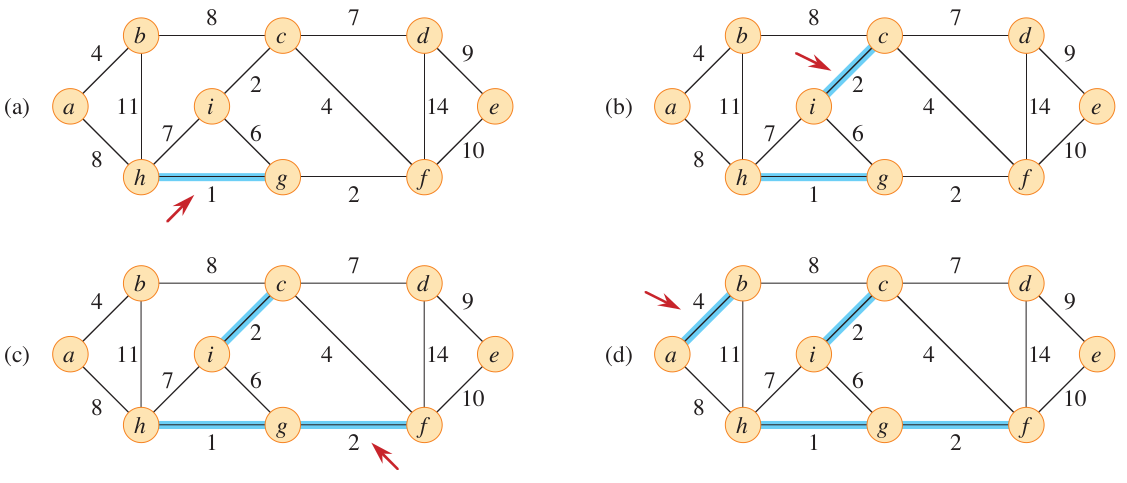
\includegraphics[width=0.7\textwidth]{figs/chap07/592-kruskal1}
\end{figure}
\end{itemize}
\end{frame}

\begin{frame}{‌الگوریتم کروسکال}
\begin{itemize}\itemr
\item[-]
\begin{figure}
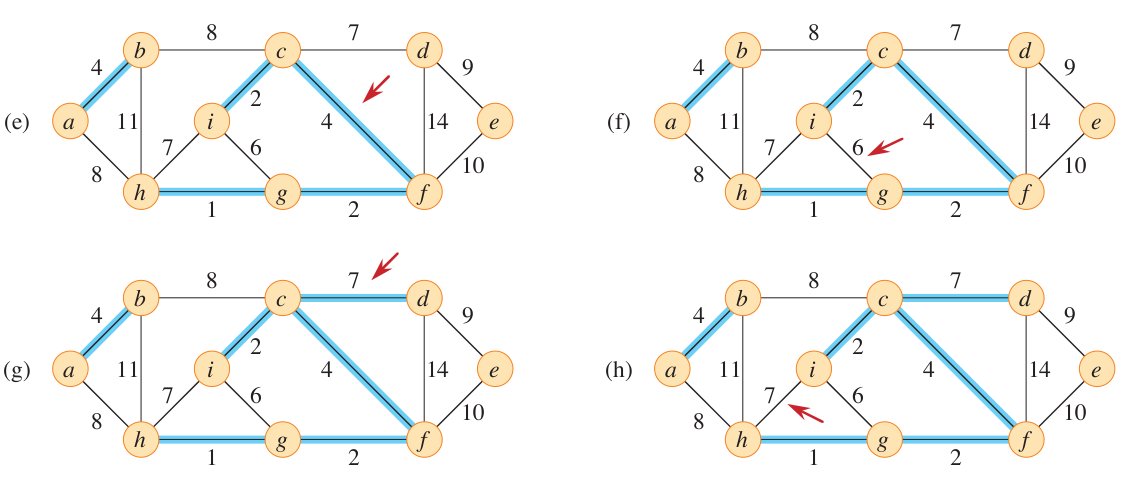
\includegraphics[width=0.7\textwidth]{figs/chap07/592-kruskal2}
\end{figure}
\end{itemize}
\end{frame}

\begin{frame}{‌الگوریتم کروسکال}
\begin{itemize}\itemr
\item[-]
\begin{figure}
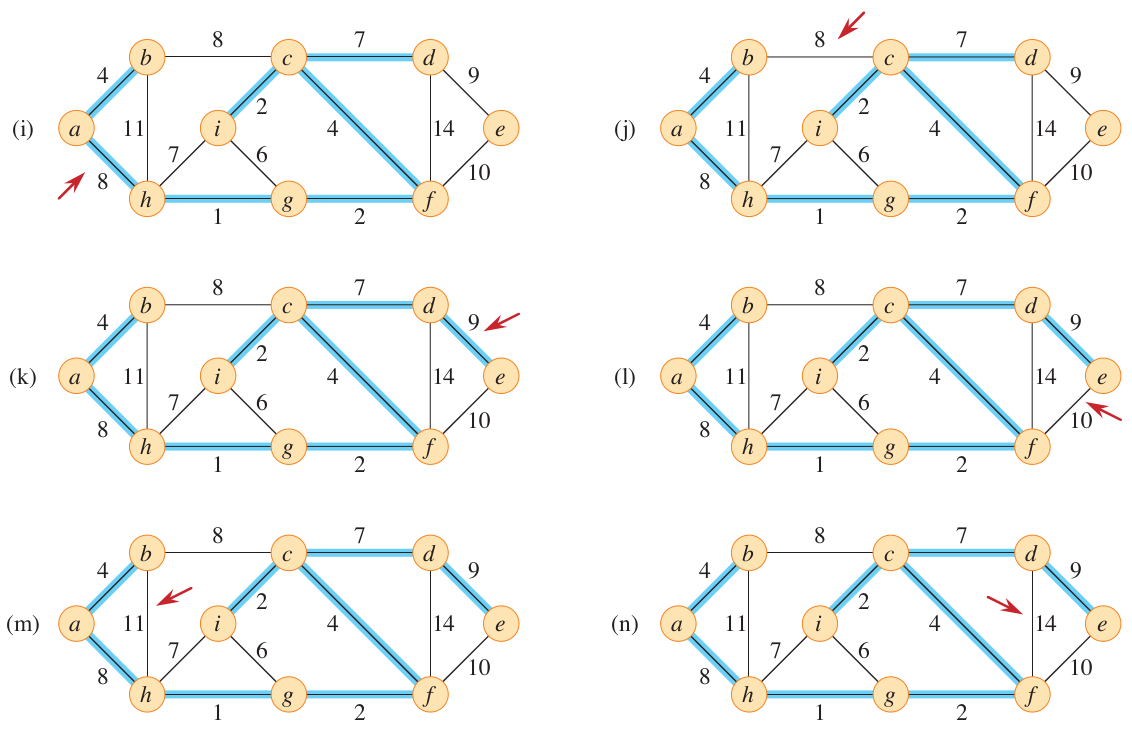
\includegraphics[width=0.7\textwidth]{figs/chap07/593-kruskal}
\end{figure}
\end{itemize}
\end{frame}


\begin{frame}{‌الگوریتم کروسکال}
\begin{itemize}\itemr
\item[-]
الگوریتم کروسکال در زیر نشان داده شده است.
\begin{algorithm}[H]\alglr
  \caption{Minimum Spanning Tree - Kruskal} 
  \begin{algorithmic}[1]
   \Func{Mst-Kruskal}{G,w}
   \State A = $\emptyset$
   \For{each vertex v $\in$ G.V}
   			\State Make-Set(v)
   	\EndFor
   	\State creat a single list of the edges in G.E
   	\State sort the list of edges into monotonically increasing order by weight w
   	\For{each edge(u,v) taken from the sorted list in order}
   			\If{Find-Set(u) $\neq$ Find-Set(v)}
   					\State A = A $\cup$ {(u,v)}
   					\State Union(Find-Set(u),Find-Set(v))
   			\EndIf
   	\EndFor
   	\State \Return A                           
  \end{algorithmic}
  \label{alg:merge}
\end{algorithm}
\end{itemize}
\end{frame}



\begin{frame}{‌الگوریتم کروسکال}
\begin{itemize}\itemr
\iffalse
\item[-]
مقدار دهی اولیه مجموعه
\m{A}
در زمان
\m{O(1)}
انجام می‌شود.
\item[-]
ساختن لیست یال‌ها در خط‌ ۴ در زمان
\m{O(V+E)}
انجام می‌شود. برای گراف همبند
\m{G}
این کار در
\m{O(E)}
انجام می‌شود.
\fi
\item[-]
در الگوریتم کروسکال،
زمان لازم برای مرتب‌سازی یال‌ها
\m{O(|E|lg|E|)}
است.
\item[-]
زمان لازم برای بررسی همهٔ یال‌ها
\m{O(|E|)}
است.
\item[-]
بنابراین، زمان اجرای الگوریتم کروسکال در مجموع
\m{O(|E|lg|E|)}
است.
\item[-]
همچنین با توجه به اینکه
\m{|E| < |V|^2}
، داریم
\m{lg|E| < 2lg|V|}
و بنابراین
\m{lg|E| = O(lg|V|)} .
پس می‌توانیم بگوییم زمان اجرای الگوریتم کروسکال برابراست با
\m{O(|E|lg|V|)} .
\end{itemize}
\end{frame}


\begin{frame}{‌کوتاهترین مسیر از یک مبدأ}
\begin{itemize}\itemr
\item[-]
فرض کنید می‌خواهیم از شهری به شهر دیگر برویم و برای کاهش هزینه می‌خواهیم کوتاهترین مسیر را انتخاب کنیم.
اطلاعات همهٔ راه‌ها و شهرها و فاصلهٔ بین شهر‌ها را در اختیار داریم. چگونه می‌توانیم با این اطلاعات کوتاهترین مسیر را انتخاب کنیم؟
\item[-]
یک راه ساده این است که همهٔ مسیرها را به دست آورده و طول آنها را با یکدیگر مقایسه کنیم، اما زمان لازم برای انجام چنین الگوریتم آنقدر زیاد است که در عمل مورد استفاده نیست.
\item[-]
در اینجا الگوریتمی برای محاسبهٔ جواب این مسئله به طور کارامد ارائه می‌کنیم.
\end{itemize}
\end{frame}


\begin{frame}{‌کوتاهترین مسیر از یک مبدأ}
\begin{itemize}\itemr
\item[-]
ورودی مسئلهٔ کوتاهترین مسیر
\fn{1}{shortest path problem},
گراف جهت‌دار وزن‌دار
\m{G = (V,E)}
با تابع وزن
\m{w : E \rightarrow \RR}
است که به ازای هر یال وزن آن را باز می‌گرداند. وزن مسیر
\m{p = \langle v_0,v_1, \cdots , v_k \rangle}
که به صورت
\m{w(p)}
نشان داده می‌شود برابراست با مجموع وزن همهٔ یال‌های مسیر:
\begin{align*}
\m{w(p) = \sum_{i = 1}^k w(v_{i-1},v_i)}
\end{align*}
\item[-]
وزن کوتاهترین مسیر از رأس
\m{u}
به
\m{v}
را به صورت زیر تعریف می‌کنیم.
\begin{align*}
\m{\delta(u,v)} = \left\{ \begin{array}{lr}
							 \m{\min \{ w(p) : u \stackrel{p}{\leadsto} v\}} & \text{اگر مسیری از u به v وجود داشته باشد}\\
							 \m{\infty} & \text{در غیر اینصورت}
							 \end{array}\right.
\end{align*}
\end{itemize}
\end{frame}


\begin{frame}{‌کوتاهترین مسیر از یک مبدأ}
\begin{itemize}\itemr
\item[-]
کوتاهترین مسیر از رأس
\m{u}
به
\m{v}
مسیر
\m{p}
است که وزن آن برابر با وزن کوتاهترین مسیر از
\m{u}
به
\m{v}
باشد :
\m{w(p) = \delta(u,v)}
\item[-]
در مثال پیدا کردن مسیر بین دو شهر، شهرها رأس‌های گراف، و جاده‌های بین دو شهر یال‌های گراف و فاصله جاده‌های بین دو شهر وزن یال‌ها هستند.
\item[-]
الگوریتم جستجوی سطح‌اول در واقع یک الگوریتم کوتاهترین مسیر برای یک گراف بدون وزن است یعنی گرافی که در آن وزن یال‌ها برابر با مقدار واحد است.
\end{itemize}
\end{frame}


\begin{frame}{‌کوتاهترین مسیر از یک مبدأ}
\begin{itemize}\itemr
\item[-]
در الگوریتم‌های کوتاهترین مسیر از روشی به نام آزادسازی
\fn{1}{relaxation}
استفاده می‌کنیم.
\item[-]
به ازای هر رأس
\m{v \in V}
الگوریتم کوتاهترین مسیر از یک رأس
\fn{2}{single-source shortest path}
یک متغیر به نام
\m{v.d}
نگه‌می‌دارد که یک کران بالا برای کوتاهترین مسیر از
\m{s}
به
\m{v}
است.
\item[-]
مقدار
\m{v.d}
را تخمین کوتاهترین مسیر
\fn{3}{shortest-path estimate}
می‌نامیم.
\end{itemize}
\end{frame}


\begin{frame}{‌کوتاهترین مسیر از یک مبدأ}
\begin{itemize}\itemr
\item[-]
برای مقداردهی اولیه تخمین فاصله و رئوس پدر هر رأس در مسئله کوتاهترین مسیر به صورت زیر عمل می‌کنیم.
\begin{algorithm}[H]\alglr
  \caption{Initialize-Single-Source} 
  \begin{algorithmic}[1]
   \Func{Initialize-Single-Source}{G,s}
   \For{each vertex v $\in$ G.V}
   			\State v.d = $\infty$
   			\State v.pred = Nil
   	\EndFor
   	\State s.d = 0   
  \end{algorithmic}
  \label{alg:merge}
\end{algorithm}
\end{itemize}
\end{frame}


\begin{frame}{‌کوتاهترین مسیر از یک مبدأ}
\begin{itemize}\itemr
\item[-]
با فرض اینکه کوتاهترین مسیر از مبدأ 
\m{s}
 به رأس
\m{u}
محاسبه شده است و 
\m{u.d}
به دست آمده است،
روند آزادسازی یال
\m{(u,v)}
بدین صورت است که بررسی می‌کنیم آیا با عبور از
\m{u}
کوتاهترین مسیر از
\m{s}
به
\m{v}
بهبود پیدا می‌کند یا خیر. اگر مقدار کوتاهترین مسیر بهبود پیدا می‌کند
\m{v.d}
و
\m{v.pred}
را به روز رسانی می‌کنیم.
\item[-]
الگوریتم آزادسازی در زیر نشان داده شده است.
\begin{algorithm}[H]\alglr
  \caption{Relax} 
  \begin{algorithmic}[1]
   \Func{Relax}{u,v,w}
   \If{v.d > u.d + w(u,v)}
   			\State v.d = u.d + w(u,v)
   			\State v.pred = u
   	\EndIf                           
  \end{algorithmic}
  \label{alg:merge}
\end{algorithm}
\end{itemize}
\end{frame}


\begin{frame}{‌کوتاهترین مسیر از یک مبدأ}
\begin{itemize}\itemr
\item[-]
در شکل زیر دو مثال از آزادسازی یک یال نشان داده شده است. در یکی از مثال‌ها تخمین کوتاهترین مسیر کاهش پیدا می‌کند و در مثال دیگر تغییری پیدا نمی‌کند.
\begin{figure}
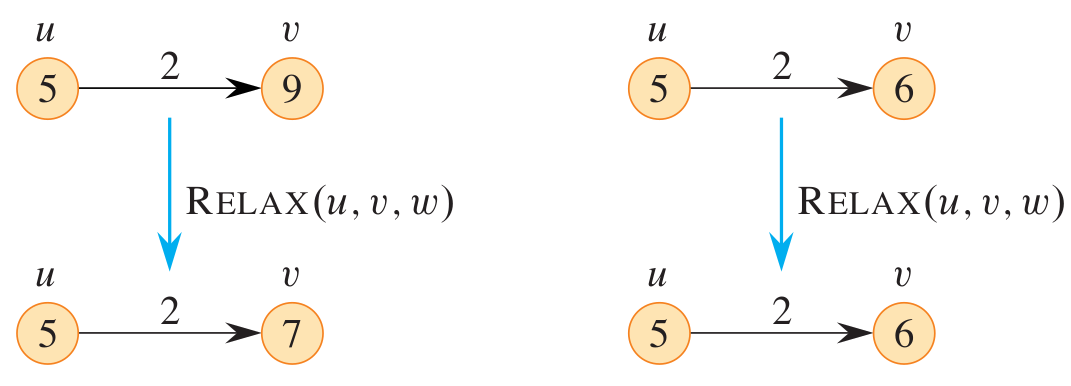
\includegraphics[width=0.7\textwidth]{figs/chap07/610-relaxation}
\end{figure}
\end{itemize}
\end{frame}


\begin{frame}{‌کوتاهترین مسیر از یک مبدأ}
\begin{itemize}\itemr
\item[-]
دو الگوریتم مهم برای محاسبه کوتاهترین مسیر عبارتند از الگوریتم بلمن فورد و الگوریتم دایکسترا.
\item[-]
در الگوریتم بلمن فورد هر یال
\m{|V| - 1}
بار آزادسازی می‌شود، اما در الگوریتم دایکسترا هر یال فقط یک بار آزادسازی می‌شود.
\item[-]
در الگوریتم بلمن‌فورد وزن یال‌ها می‌توانند منفی نیز باشد، اما الگوریتم دایکسترا تنها گراف‌هایی با وزن یال مثبت را می‌پذیرد.
وزن یال منفی می‌تواند کاربردهای متنوعی داشته باشد. برای مثال، اگر یک خودروی برقی را در نظر بگیریم که در جاده‌هایی با شیب منفی شارژ می‌شود و در جاده‌هایی با شیب مثبت انرژی مصرف می‌کند، می‌توانیم شیب جاده را به عنوان وزن یال‌های گراف در نظر بگیریم.
\end{itemize}
\end{frame}

\begin{frame}{‌الگوریتم بلمن-فورد}
\begin{itemize}\itemr
\item[-]
الگوریتم بلمن-فورد
\fn{1}{Bellman-Ford algorithm}
مسئله کوتاهترین مسیر را در حالت کلی حل می‌کند وقتی وزن یال‌ها می‌توانند منفی نیز باشند.
\item[-]
به ازای یک گراف دلخواه
\m{G = (V,E)}
با یال‌های وزن‌دار و رأس مبدأ
\m{s}
و تابع وزن
\m{w : E \rightarrow \RR}
الگوریتم بلمن فورد در صورتی که یک دور با وزن منفی وجود داشته باشد که از مبدأ قابل دسترسی باشد، مقدار نادرست را باز می‌گرداند، بدین معنی که کوتاهترین مسیر وجود ندارد. اما اگر چنین دوری وجود نداشته باشد، الگوریتم بلمن فورد کوتاهترین مسیر را از مبدأ به همهٔ رئوس را باز می‌گرداند.
\end{itemize}
\end{frame}


\begin{frame}{‌الگوریتم بلمن-فورد}
\begin{itemize}\itemr
\item[-]
الگوریتم بلمن فورد در زیر توصیف شده است.
\begin{algorithm}[H]\alglr
  \caption{Bellman-Ford} 
  \begin{algorithmic}[1]
   \Func{Bellman-Ford}{G,w,s}
   \State Initialize-Single-Source(G, s)
   \For{i = 1 \To |G.V| - 1}
   		\For{each edge (u,v) $\in$ G.E}
   				\State Relax(u,v,w)
   		\EndFor
   	\EndFor
   	\For{each edge (u,v) $\in$ G.E}
   			\If{v.d > u.d + w(u,v)}
   					\State \Return False
   			\EndIf
   	\EndFor
   	\State \Return True                         
  \end{algorithmic}
  \label{alg:merge}
\end{algorithm}
\end{itemize}
\end{frame}


\begin{frame}{‌الگوریتم بلمن-فورد}
\begin{itemize}\itemr
\item[-]
یک مثال از اجرای الگوریتم بلمن فورد در زیر نشان داده شده است.
\begin{figure}
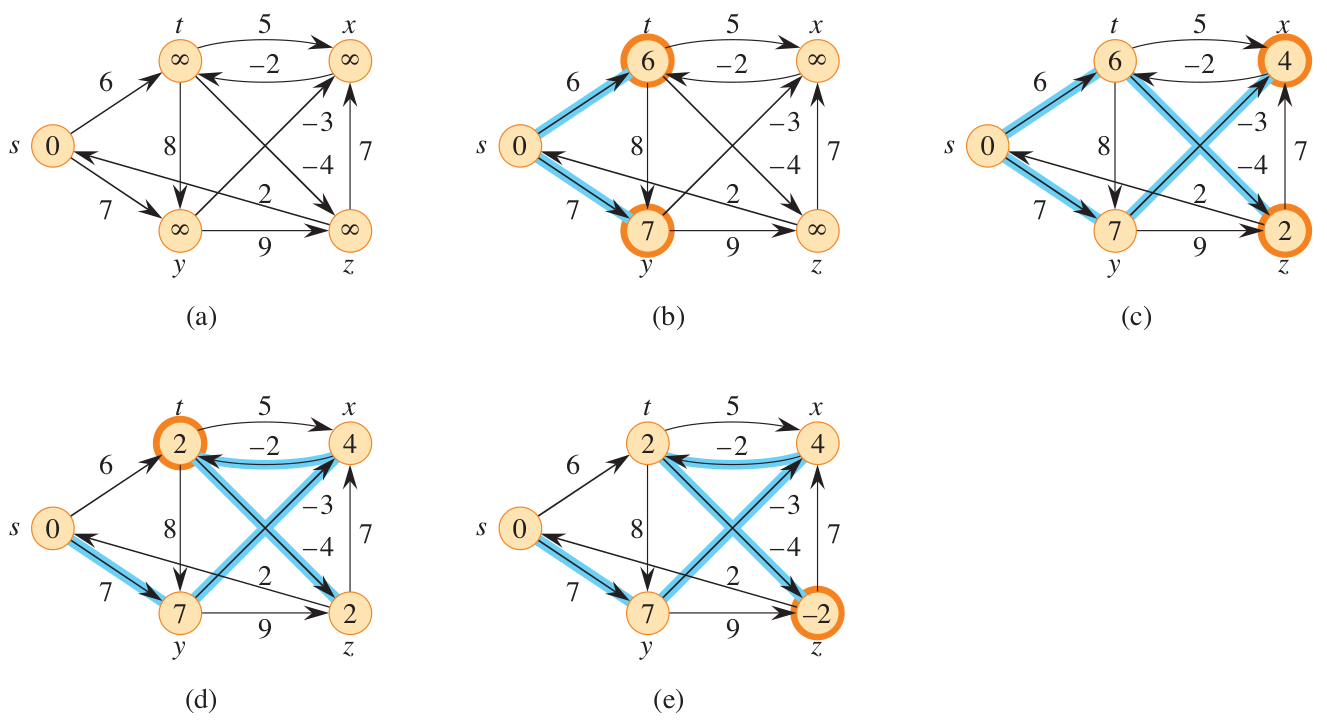
\includegraphics[width=0.7\textwidth]{figs/chap07/613-bellman}
\end{figure}
\end{itemize}
\end{frame}


\begin{frame}{‌الگوریتم بلمن-فورد}
\begin{itemize}\itemr
\item[-]
مقداردهی اولیه در خط ۱ در زمان
\ath{|V|}
اجرا می‌شود.
\item[-]
%اگر گراف با لیست مجاورت نمایش داده شود،
بررسی همهٔ یال‌ها به زمان 
\ath{|E|}
نیاز خواهد داشت.
% وقتی که گراف با لیست مجاورت نمایش داده شده باشد.
\item[-]
در حلقه خطوط ۲ تا ۴ هر یک از
\m{|V| -1}
تکرارهای حلقه، در زمان
\ath{|E|}
اجرا می‌شود.
\item[-]
حلقه خطوط ۵ تا ۷ در زمان
\ath{|E|}
اجرا می‌شود.
\item[-]
بنابراین الگوریتم بلمن فورد در زمان
\m{O(|V| |E|)}
اجرا می‌شود.

\end{itemize}
\end{frame}

\begin{frame}{‌الگوریتم بلمن-فورد}
\begin{itemize}\itemr
\item[-]
برای اثبات درستی الگوریتم بلمن فورد نشان می‌دهیم اگر هیچ دوری با وزن منفی وجود نداشته باشد، این الگوریتم به درستی کوتاهترین مسیر را برای همهٔ رئوس از یک رأس مبدأ محاسبه می‌کند.
\item[-]
قضیه:
فرض کنید
\m{G = (V,E)}
یک گراف وزن‌دار جهت‌دار با رأس مبدأ
\m{s}
و تابع وزن
\m{w : E \rightarrow \RR}
باشد و فرض کنید
\m{G}
هیچ دوری با وزن منفی نداشته باشد که از
\m{s}
قابل دسترسی باشد. آنگاه بعد از
\m{|V| -1}
تکرار در حلقهٔ خطوط ۲ تا ۴ الگوریتم بلمن فورد به دست می‌آوریم
\m{v.d = \delta(s,v)}
به ازای همه رئوس
\m{v}
که از
\m{s}
قابل دسترس هستند.
\end{itemize}
\end{frame}


\begin{frame}{‌الگوریتم بلمن-فورد}
\begin{itemize}\itemr
\item[-]
اثبات : یک رأس
\m{v}
را در نظر بگیرید که از
\m{s}
قابل دسترس است و فرض کنید
\m{p = \langle v_0,v_1, \cdots , v_k \rangle}
به طوری‌که
\m{v_0 = s}
و
\m{v_k = v}
و
\m{p}
کوتاهترین مسیر از
\m{s}
به
\m{v}
باشد.
\item[-]
از آنجایی که کوتاهترین مسیر باید یک مسیر ساده باشد،
\m{p}
حداکثر
\m{|V| -1}
یال دارد و بنابراین
\m{k \leqslant |V| -1} .
\item[-]
هر یک از
\m{|V| -1}
تکرار در حلقه خطوط ۲ تا ۴ همه
\m{|E|}
یال را آزادسازی می‌کند.
\end{itemize}
\end{frame}


\begin{frame}{‌الگوریتم بلمن-فورد}
\begin{itemize}\itemr
\item[-]
بعد از یک بار تکرار حلقه، یال
\m{(s,v_1)}
آزاد سازی می‌شود و بنابراین
\m{v_1.d = w(s,v_1) = \delta(s, v_1)}
وزن کوتاهترین مسیر از
\m{s}
به
\m{v_1}
خواهد بود.
\item[-]
بعد از دو بار تکرار حلقه، یال
\m{(v_1,v_2)}
برای بار دوم آزادسازی می‌شود
 بنابراین
\m{v_2.d = v_1.d + w(v_1,v_2) = \delta(s,v_2)}
وزن کوتاهترین مسیر از
\m{s}
به
\m{v_2}
خواهد بود.
\item[-]
بنابراین
 در تکرار
\m{i}
ام، به ازای
\m{i = 1,2, \cdots, k}
یال
\m{(v_{i-1},v_i)}
 آزادسازی می‌شود و  
\m{v_i.d = v_{i-1}.d + w(v_{i-1},v_i) = \delta(s, v_i)}
وزن کوتاهترین مسیر از
\m{s}
به
\m{v_i}
خواهد بود.
\item[-]
 پس از 
\m{|V| -1}
بار آزادسازی یال‌ها
به دست می‌آوریم:
\begin{align*}
\m{v_k.d = \delta(s,v_k)}
\end{align*}
\end{itemize}
\end{frame}


\iffalse
\begin{frame}{‌الگوریتم بلمن-فورد}
\begin{itemize}\itemr
\item[-]
ویژگی آزادسازی مسیر
\fn{1}{path relaxation property}
به صورت زیر است.
\item[-]
اگر
\m{p = \langle v_0,v_1, \cdots , v_k \rangle}
کوتاهترین مسیر از
\m{s = v_0}
به
\m{v_k}
باشد و یال‌های
\m{p}
به ترتیب
\m{(v_0,v_1)}
،
\m{(v_1,v_2)}
،
\m{\cdots}
،
\m{(v_{k-1},v_k)}
آزادسازی شوند، آنگاه
\m{v_{k}.d = \delta(s,v_k)}
\end{itemize}
\end{frame}
\fi

\begin{frame}{‌الگوریتم دایکسترا}
\begin{itemize}\itemr
\item[-]
الگوریتم دایکسترا مسئله کوتاهترین مسیر برای گراف وزن‌دار جهت‌دار
\m{G = (V,E)}
را وقتی وزن‌ها منفی نباشند حل می‌کند. به عبارت دیگر به ازای هر یال
\m{(u,v) \in E}
در الگوریتم دایکسترا لازم است داشته باشیم
\m{w(u,v) \geqslant 0} .
\item[-]
با یک پیاده‌سازی بهینه، الگوریتم دایکسترا می‌تواند در زمان کمتری نسبت به الگوریتم بلمن-فورد مسئله را حل کند.
\end{itemize}
\end{frame}


\begin{frame}{‌الگوریتم دایکسترا}
\begin{itemize}\itemr
\item[-]
الگوریتم دایکسترا به صورت زیر است.
\begin{algorithm}[H]\alglr
  \caption{Dijkstra} 
  \begin{algorithmic}[1]
  \Func{Dijkstra}{G, w, s}
   \State Initialize-Single-Source(G,s)
   \State S = $\emptyset$
   \State Q = $\emptyset$
   \For{each vertex u $\in$ G.V}
   		\State Insert(Q,u)
   	\EndFor
   	\While{Q $\neq \emptyset$}
   			\State u = Extract-Min(Q)
   			\State S = S $\cup$ \{u\}
   			\For{each vertex v in G.Adj[u]}
   					\State Relax(u,v,w)
   					\If{the call of Relax decreased v.d}
   							\State Decrease-Key(Q,v,v.d)
   					\EndIf
   			\EndFor
   	\EndWhile                       
  \end{algorithmic}
  \label{alg:merge}
\end{algorithm}
\end{itemize}
\end{frame}


\begin{frame}{‌الگوریتم دایکسترا}
\begin{itemize}\itemr
\item[-]
یک مثال از الگوریتم دایکستر در شکل زیر نشان داده شده است.
\begin{figure}
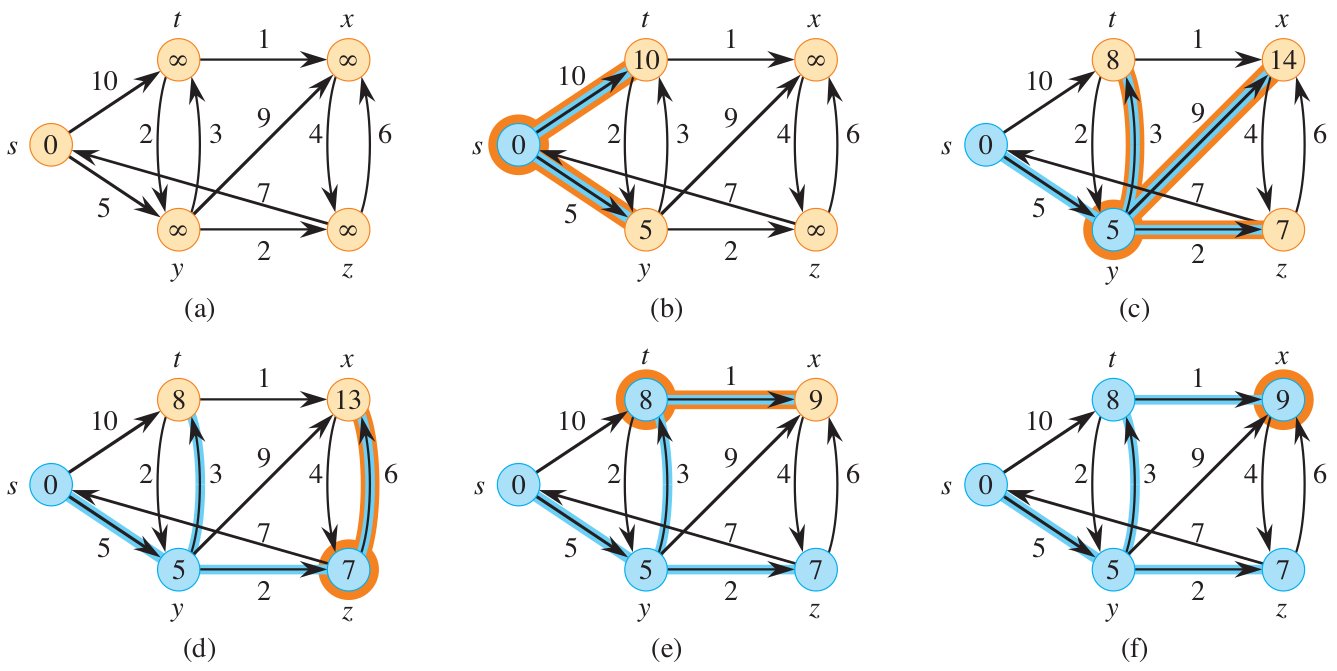
\includegraphics[width=0.9\textwidth]{figs/chap07/621-dijkstra}
\end{figure}
\end{itemize}
\end{frame}


\begin{frame}{‌الگوریتم دایکسترا}
\LR{
\begin{figure}[!ht]
 % \centering
  {\includestandalone[width=0.22\textwidth]{figs/chap07/d1}}
 {\includestandalone[width=0.22\textwidth]{figs/chap07/d2}}
 {\includestandalone[width=0.22\textwidth]{figs/chap07/d3}}
  {\includestandalone[width=0.22\textwidth]{figs/chap07/d4}}
  {\includestandalone[width=0.22\textwidth]{figs/chap07/d5}}
  {\includestandalone[width=0.22\textwidth]{figs/chap07/d6}}
 {\includestandalone[width=0.22\textwidth]{figs/chap07/d7}}
  {\includestandalone[width=0.22\textwidth]{figs/chap07/d8}}
  \iffalse
 \only<1>{\includestandalone{figs/chap07/d1}}
 \only<2>{\includestandalone{figs/chap07/d2}}
 \only<3>{\includestandalone{figs/chap07/d3}}
  \only<4>{\includestandalone{figs/chap07/d4}}
  \only<5>{\includestandalone{figs/chap07/d5}}
  \only<6>{\includestandalone{figs/chap07/d6}}
  \only<7>{\includestandalone{figs/chap07/d7}}
  \only<8>{\includestandalone{figs/chap07/d8}}
  \fi
  \label{fig:d1}
\end{figure}
}
\iffalse
\[
P =~\langle~c_1, \pause \pause c_2, \pause \pause c_3,\pause \pause 
c_4,  \pause c_5 ~\rangle
\]
\fi
\end{frame}



\begin{frame}{‌الگوریتم دایکسترا}
\begin{itemize}\itemr
\item[-]
مجموعهٔ 
\m{S}
شامل رئوسی است که کوتاهترین مسیر از مبدأ برای آنها تعیین شده است.
\item[-]
از آنجایی که الگوریتم دایکسترا همیشه نزدیک‌ترین رأس به مبدأ در
\m{V-S}
را به
\m{S}
اضافه می‌کند، این الگوریتم یک الگوریتم حریصانه است.
\end{itemize}
\end{frame}


\begin{frame}{‌الگوریتم دایکسترا}
\begin{itemize}\itemr
\item[-]
برای تحلیل زمان اجرای الگوریتم دایکسترا از تحلیل تجمعی استفاده می‌کنیم.
\item[-]
از آنجایی که هر رأس
\m{u \in V}
به مجموعهٔ
\m{S}
فقط یک‌بار اضافه می‌شود، هر یال در لیست مجاورت
\m{Adj[u]}
در حلقه
\code{for}
خطوط ۹ تا ۱۲ دقیقا یک‌بار در طول اجرای الگوریتم بررسی می‌شود.
بنابراین این حلقه در مجموع
به تعداد یال‌های گراف
تکرار می‌شود و
\code{Decrease-key}
در مجموع حداکثر
به تعداد یال‌ها
تکرار می‌شود.
هزینه بررسی همهٔ یال‌ها
\m{O(|E|)}
است.
\item[-]
حلقه
\code{while}
نیز به تعداد رئوس گراف تکرار می‌شود.
\item[-]
زمان اجرای الگوریتم دایکسترا به پیاده‌سازی صف اولویت بستگی پیدا می‌کند.
\item[-]
در یک پیاده‌سازی ساده صف اولویت توابع
\code{Insert}
و
\code{Decrease-key}
در زمان
\m{O(1)}
و تابع
\code{Extract-Min}
در زمان
\m{O(|V|)}
اجرا می‌شود.
\item[-]
بنابراین زمان اجرای الگوریتم
\m{O(|V|^2 + |E|) = O(|V|^2)}
است.
\end{itemize}
\end{frame}



\begin{frame}{‌الگوریتم دایکسترا}
\begin{itemize}\itemr
\item[-]
اگر صف اولویت با استفاده از هیپ پیاده‌سازی شود،
 توابع
\code{Extract-Min}
و
\code{Decrease-key}
در زمان
\m{O(lg|V|)}
اجرا می‌شوند.
\item[-]
بنابراین زمان اجرای الگوریتم
\m{O((|V|+|E|)lg|V|)}
خواهد بود.
\item[-]
در یک گراف همبند که تعداد یال‌ها بزرگتر یا مساوی تعداد رئوس است، الگوریتم دایکسترا در زمان
\m{O(|E| lg |V|)}
اجرا می‌شود.
\item[-]
یک پیاده‌سازی بهینه‌تر نیز با استفاده از هرم فیبوناچی برای الگوریتم دایکسترا وجود دارد که زمان اجرا را به
\m{O(|E| + |V| lg |V|)}
کاهش می‌دهد که در اینجا به آن نمی‌پردازیم.
\end{itemize}
\end{frame}

\begin{frame}{‌کوتاهترین مسیر بین همهٔ جفت‌ها}
\begin{itemize}\itemr
\item[-]
اکنون مسئله کوتاهترین مسیر بین همهٔ جفت رأس‌ها در گراف را بررسی می‌کنیم.
\item[-]
یکی از کاربرهای این الگوریتم، پیدا کردن کوتاهترین مسیر بین هر دو شهر در یک اطلس جغرافیایی است. یکی از کاربردهای دیگر این الگوریتم پیدا کردن فاصلهٔ بین دو نقطه در یک شبکه کامپیوتری برای ارسال بسته‌ها به طور بهینه است.
\item[-]
خروجی الگوریتم یک جدول به اندازهٔ
\m{|V| \times |V|}
است که در سطر
\m{u}
و ستون
\m{v}
فاصله بین شهر
\m{u}
و شهر
\m{v}
را باز می‌گرداند.
\end{itemize}
\end{frame}


\begin{frame}{‌کوتاهترین مسیر بین همهٔ جفت‌ها}
\begin{itemize}\itemr
\item[-]
یک راه حل ساده این است که به ازای هر یک از رئوس گراف، آن رأس را مبدأ فرض کرده و الگوریتم کوتاهترین مسیر از رأس مبدأ را از هریک از رئوس گراف اجرا کنیم تا فاصله بین همهٔ رئوس به دست بیاید برای مثال اگر وزن یال‌ها مثبت باشند، می‌توان از الگوریتم دایکسترا به تعداد
\m{|V|}
بار استفاده کرد که در مجموع کل محاسبات در زمان
\m{O(|V|^3)}
 اجرا می‌شود.
اگر صف اولویت در الگوریتم دایکسترا توسط هرم فیبوناچی پیاده‌سازی شود، زمان اجرا به
\m{O(|V|^2 lg |V| + |V||E|)}
کاهش پیدا می‌کند.
البته در بدترین حالت 
\m{|E| = O(|V|^2)},
بنابراین زمان اجرای الگوریتم یافتن کوتاهترین مسیر بین همه جفت رئوس با استفاده از الگوریتم دایکسترا برابر است با 
\m{O(|V|^3)} .
\item[-]
اگر گراف یال‌هایی با وزن منفی داشته باشد، نمی‌توان از الگوریتم دایکسترا استفاده کرد. می‌توانیم در این‌صورت با استفاده از الگوریتم بلمن-فورد، کوتاهترین مسیر بین همهٔ جفت‌ها را در زمان
\m{O(|V|^2 |E|)}
محاسبه کنیم که در صورتی که گراف متراکم باشد، زمان اجرا برابر خواهد بود با
\m{O(|V|^4)} .
\end{itemize}
\end{frame}


\begin{frame}{‌کوتاهترین مسیر بین همهٔ جفت‌ها}
\begin{itemize}\itemr
\item[-]
در این قسمت الگوریتمی ارائه می‌کنیم که کوتاهترین مسیر بین همهٔ رئوس را در زمان کمتری محاسبه کند.
\item[-]
برای استفاده از این الگوریتم، گراف را با استفاده از ماتریس مجاورت نشان می‌دهیم.
\end{itemize}
\end{frame}


\begin{frame}{‌کوتاهترین مسیر بین همهٔ جفت‌ها}
\begin{itemize}\itemr
\item[-]
اگر رأس‌ها را با شماره‌های ۱، ۲، ... ،
\m{|V|}
شماره گذاری کنیم، به طوری‌که تعداد رئوس برابر با
\m{n}
باشد، آنگاه یک ماتریس
\m{n \times n}
که با
\m{W = (w_{ij})}
نشان می‌دهیم، وزن یال‌ها را در گراف
\m{G = (V,E)}
نشان می‌دهد، به طوری‌که
\begin{align*}
\m{w_{ij}} = \left\{\begin{array}{llr}
          \m{0}& \m{i = j}&\text{اگر}\\
          \m{w(i,j)}&\m{(i,j) \in E}~\text{و}~\m{i \neq j}&\text{اگر}\\
          \m{\infty}&\m{(i,j) \notin E}&\text{اگر}
\end{array}\right.
\end{align*}
\item[-]
خروجی الگوریتم یک جدول
\m{n \times n}
خواهد بود به طوری‌که در سطر
\m{i}
و ستون
\m{j}
مقدار
\m{\delta(i,j)}
قرار گیرد.
\item[-]
خروجی الگوریتم کوتاهترین مسیر می‌تواند شامل یک ماتریس رئوس ماقبل
\fn{1}{predecessor matrix}
به نام
\m{\Pi = (\pi_{ij})}
نیز باشد که در آن
\m{\pi_{ij}}
رأس پدر (ماقبل) رأس
\m{j}
را بر روی مسیری که از رأس
\m{i}
آغاز شده نشان می‌دهد. در صورتی که
\m{i = j}
باشد یا هیچ مسیری از
\m{i}
به
\m{j}
وجود نداشته باشد، آنگاه
\m{\pi_{ij}}
برابر با
\code{NIL}
خواهد بود.
\end{itemize}
\end{frame}


\begin{frame}{‌کوتاهترین مسیر بین همهٔ جفت‌ها}
\begin{itemize}\itemr
\item[-]
برای چاپ کوتاهترین مسیر از
\m{i}
به
\m{j}
با استفاده از ماتریس رئوس ماقبل می‌توانیم از الگوریتم زیر استفاده کنیم.
\begin{algorithm}[H]\alglr
  \caption{Print-All-Pairs-Shortest-Path} 
  \begin{algorithmic}[1]
   \Func{Print-All-Pairs-Shortest-Path}{\mc{\Pi},i,j}
   \If{i == j}
   		\State print i
   \ElsIf{\mc{\pi_{ij}} == NIL}
   		\State print "no path from" i "to" j "exists"
   \Else
        \State Print-All-Pairs-Shortest-Path(\mc{\Pi},i,\mc{\pi_{ij}})
   		\State print j
   \EndIf                           
  \end{algorithmic}
  \label{alg:merge}
\end{algorithm}
\end{itemize}
\end{frame}

\begin{frame}{‌الگوریتم فلوید-وارشال}
\begin{itemize}\itemr
\item[-]
الگوریتم فلوید-وارشال
\fn{1}{Floyed-Warshall algorithm}
مسئله کوتاهترین مسیر بین همهٔ جفت‌ها را در زمان
\m{O(V^3)}
حل می‌کند. در این الگوریتم یال‌ها با وزن منفی می‌توانند وجود داشته باشند، اما دورها با وزن منفی در گراف ورودی مسئله مجاز نیستند.
این الگوریتم یک الگوریتم از نوع برنامه‌ریزی پویا است.
\end{itemize}
\end{frame}


\begin{frame}{‌الگوریتم فلوید-وارشال}
\begin{itemize}\itemr
\item[-]
رئوس گراف
\m{G}
را با اعداد صحیح شماره گذاری می‌کنیم. بنابراین خواهیم داشت
\m{V = \{1,2, \cdots, n\}} .
\item[-]
برای حل این مسئله با استفاده از برنامه‌ریزی پویا ابتدا کوتاهترین مسیر بین رئوس 
\m{i}
و
\m{j}
را با فرض اینکه
هیچ رأسی در مسیر وجود نداشته باشد محاسبه می‌کنیم. در صورتی که یال
\m{(i,j)}
وجود داشته باشد، طول چنین مسیری برابر با وزن این یال است.
سپس کوتاهترین مسیر بین رئوس
\m{i}
و
\m{j}
را با فرض بر اینکه
 فقط رأس 
\m{1}
در مسیر
 وجود داشته باشد به دست می‌آوریم. سپس فرض می‌کنیم رأس 
\m{2}
  نیز وجود داشته باشد
و کوتاهترین مسیر بین همهٔ جفت رئوس را با فرض اینکه رئوس میانی مسیر
در مجموعهٔ
\m{\{1, 2 \}}
باشند محاسبه می‌کنیم.
\item[-]
 به همین ترتیب 
به ازای
\m{1 \leqslant k \leqslant n}
زیر مجموعهٔ
\m{\{1,2, \cdots, k\}}
از رئوس را در نظر می‌گیریم و به ازای هر جفت از رئوس
\m{i,j \in V}
، همه مسیرها از
\m{i}
به
\m{j}
را که از رئوس
\m{\{1,2, \cdots, k\}}
می‌گذرند را در نظر می‌گیریم و فرض می‌کنیم
\m{p}
کوتاهترین مسیر بین همهٔ این مسیرها باشد.
\end{itemize}
\end{frame}


\begin{frame}{‌الگوریتم فلوید-وارشال}
\begin{itemize}\itemr
\item[-]
حال حالت‌های زیر را در نظر می‌گیریم.
\item[-]
اگر
\m{k}
یک رأس میانی در مسیر
\m{p}
نباشد، آنگاه همهٔ رئوس میانی مسیر
\m{p}
متعلق به مجموعهٔ
\m{\{1,2, \cdots, k-1\}}
هستند. بنابراین کوتاهترین مسیر از رأس
\m{i}
به رأس
\m{j}
با رئوس میانی
\m{\{1,2, \cdots, k\}} ,
همان
کوتاهترین مسیر از
\m{i}
به
\m{j}
با رئوس میانی در مجموعهٔ
\m{\{1,2, \cdots, k-1\}}
است.
\item[-]
اگر
\m{k}
یک رأس میانی در مسیر
\m{p}
باشد، آنگاه مسیر
\m{p}
را به دو قسمت
\m{i \stackrel{p_1}{\leadsto} k \stackrel{p_2}{\leadsto}j }
تقسیم می‌کنیم. 
 چون رأس
\m{k}
یک رأس میانی در مسیر
\m{p_1}
نیست، همهٔ رئوس میانی در مسیر
\m{p_1}
به مجموعهٔ
\m{\{1,2, \cdots, k-1\}}
تعلق دارند. بنابراین
\m{p_1}
کوتاهترین مسیر از
\m{i}
به
\m{k}
با همهٔ رئوس میانی
\m{\{1,2, \cdots, k-1\}}
است. همچنین
\m{p_2}
کوتاهترین مسیر از رأس
\m{k}
به رأس
\m{j}
با همهٔ رئوس میانی در مجموعهٔ
\m{\{1,2, \cdots, k-1\}}
است.
\end{itemize}
\end{frame}


\begin{frame}{‌الگوریتم فلوید-وارشال}
\begin{itemize}\itemr
\item[-]
شکل زیر این تقسیم بندی مسیر را نشان می‌دهد.
\begin{figure}
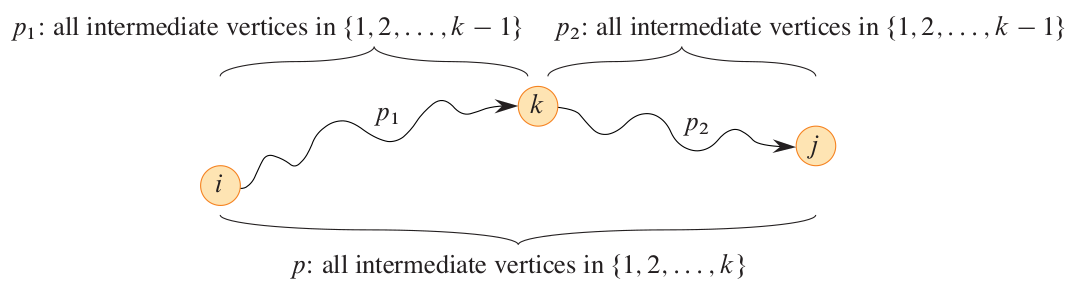
\includegraphics[width=0.9\textwidth]{figs/chap07/656-floyd}
\end{figure}
\end{itemize}
\end{frame}


\begin{frame}{‌الگوریتم فلوید-وارشال}
\begin{itemize}\itemr
\item[-]
بر اساس مشاهدهٔ قبلی می‌توانیم جواب مسئله کوتاهترین مسیر بین جفت‌ها را به صورت یک رابطهٔ بازگشتی بیان کنیم.
\item[-]
فرض کنید
\m{d_{ij}^{(k)}}
طول کوتاهترین مسیر از
\m{i}
به
\m{j}
باشد به طوری‌که رئوس میانی متعلق به مجموعه
\m{\{1,2, \cdots, k\}}
باشند.
\end{itemize}
\end{frame}


\begin{frame}{‌الگوریتم فلوید-وارشال}
\begin{itemize}\itemr
\item[-]
وقتی
\m{k = 0}
است، یک مسیر از رأس
\m{i}
به رأس
\m{j}
که هیچ رأس میانی با شماره‌ای بزرگ‌تر از
\m{0}
نداشته باشد، درواقع هیچ رأس میانی ندارد. چنین مسیری حداکثر یک یال دارد، بنابراین
\m{d_{ij}^{(0)} = w_{ij}}
\item[-]
می‌توانیم مقدار
\m{d_{ij}^{(k)}}
را به صورت بازگشتی تعریف کنیم.
\begin{align*}
\m{d_{ij}^{(k)}} = \left\{\begin{array}{lr}
          \m{w_{ij}}& \m{k = 0}~\text{اگر}\\
          \m{min\{d_{ij}^{(k-1)} , d_{ik}^{(k-1)} + d_{kj}^{(k-1)} \}}& \m{k \geqslant 1}~\text{اگر}
\end{array}\right.
\end{align*}
\item[-]
چون برای هر مسیر، همهٔ رئوس میانی متعلق به مجموعهٔ
\m{\{1,2, \cdots, k\}}
هستند، بنابراین ماتریس
\m{D^n = (d_{ij}^{(n)})}
شامل جواب پایانی است. به ازای هر
\m{i,j \in V}
داریم
\m{d_{ij}^{(n)} = \delta(i,j)} .
\end{itemize}
\end{frame}


\begin{frame}{‌الگوریتم فلوید-وارشال}
\begin{itemize}\itemr
\item[-]
الگوریتم فلوید-وارشال از رابطه بازگشتی محاسبه شده استفاده می‌کند و توسط یک روند پایین به بالا مقدار بالا
\m{d_{ij}^{(k)}}
را به ازای
\m{k}
های متفاوت از کوچک به بزرگ محاسبه می‌کند.
\end{itemize}
\end{frame}


\begin{frame}{‌الگوریتم فلوید-وارشال}
\begin{itemize}\itemr
\item[-]
گراف زیر را در نظر بگیرید.
\begin{figure}
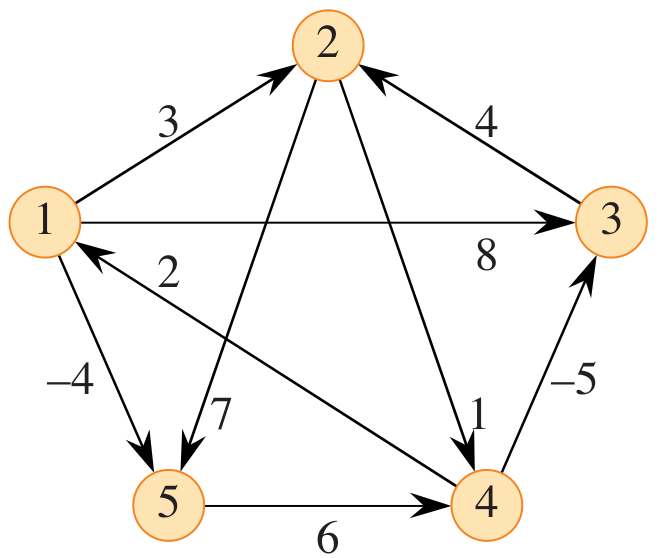
\includegraphics[width=0.4\textwidth]{figs/chap07/652-graph}
\end{figure}
\end{itemize}
\end{frame}

\begin{frame}{‌الگوریتم فلوید-وارشال}
\begin{itemize}\itemr
\item[-]
شکل زیر فرایند محاسبه ماتریس‌های
\m{D^{(k)}}
و
\m{\Pi^{(k)}}
را برای این گراف نشان می‌دهد.
\begin{figure}
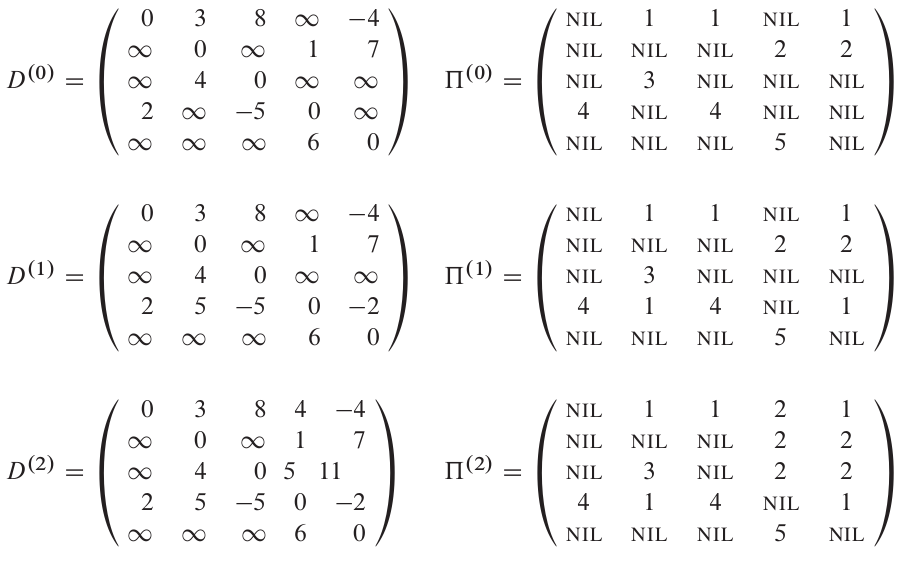
\includegraphics[width=0.6\textwidth]{figs/chap07/658-floyd-pi-1}
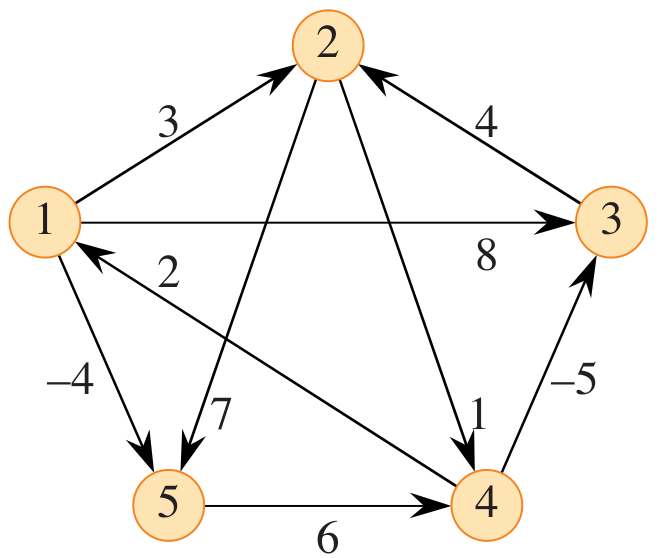
\includegraphics[width=0.3\textwidth]{figs/chap07/652-graph}
\end{figure}
\end{itemize}
\end{frame}


\begin{frame}{‌الگوریتم فلوید-وارشال}
\begin{itemize}\itemr
\item[-]
شکل زیر فرایند محاسبه ماتریس‌های
\m{D^{(k)}}
و
\m{\Pi^{(k)}}
را برای این گراف نشان می‌دهد.
\begin{figure}
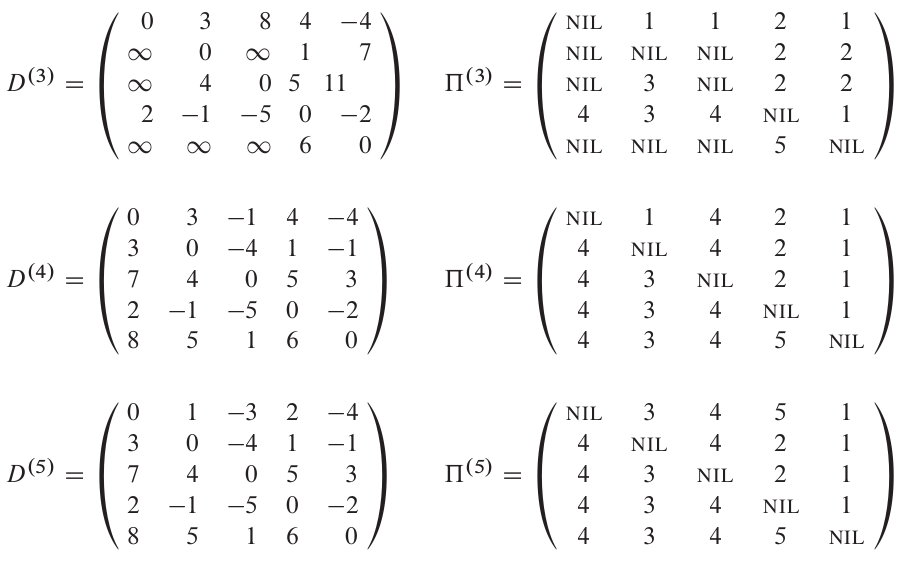
\includegraphics[width=0.6\textwidth]{figs/chap07/658-floyd-pi-2}
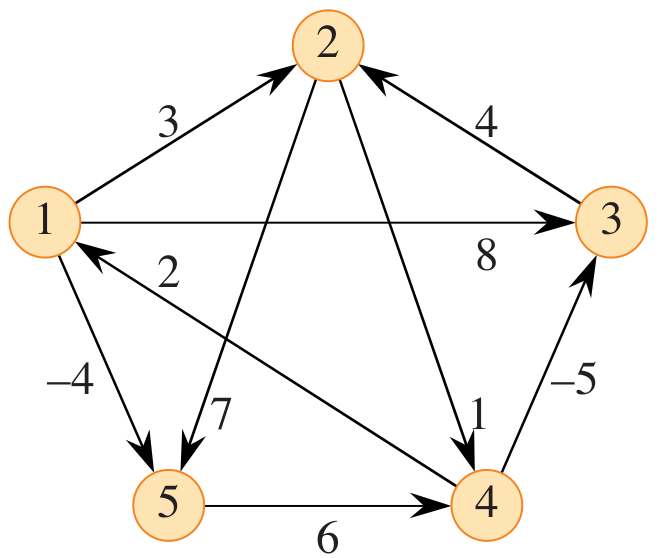
\includegraphics[width=0.3\textwidth]{figs/chap07/652-graph}
\end{figure}
\end{itemize}
\end{frame}



\begin{frame}{‌الگوریتم فلوید-وارشال}
\begin{itemize}\itemr
\item[-]
الگوریتم فلوید-وارشال به صورت زیر است.
\begin{algorithm}[H]\alglr
  \caption{Floyd-Warshall} 
  \begin{algorithmic}[1]
   \Func{Floyd-Warshall}{W,n}
   \State \mc{D^{(0)}} = W
   \For{k = 1 \To n}
   		\State let \mc{D^{(k)}} = (\mc{d_{ij}^{(k)}}) be a new n \mc{\times} n matrix
   		\For{i = 1 \To n}
   				\For{j = 1 \To n}
   						\State \mc{d_{ij}^{(k)}} = \mc{\min \{d_{ij}^{(k-1)} , d_{ik}^{(k-1)} + d_{kj}^{(k-1)}\}}
   				\EndFor
   		\EndFor
   	\EndFor
   	\State \Return \mc{D^{(n)}}                       
  \end{algorithmic}
  \label{alg:merge}
\end{algorithm}
\end{itemize}
\end{frame}


\begin{frame}{‌الگوریتم فلوید-وارشال}
\begin{itemize}\itemr
\item[-]
در الگوریتم فلوید-وارشال سه حلقه
\code{for}
تودرتو وجود دارد. چون محاسبه خط ۶ برنامه در زمان
\m{O(1)}
انجام می‌شود، بنابراین این الگوریتم در زمان
\ath{n^3}
محاسبه می‌شود.
\end{itemize}
\end{frame}


\begin{frame}{‌الگوریتم فلوید-وارشال}
\begin{itemize}\itemr
\item[-]
ماتریس رئوس ماقبل
\m{\Pi}
نیز می‌تواند در زمان محاسبهٔ
\m{D^{(0)}}
،
\m{D^{(1)}}
،
\m{\cdots}
،
\m{D^{(n)}}
محاسبه شود.
\item[-]
به عبارت دیگر می‌توانیم
\m{\Pi^{0}}
،
\m{\Pi^{1}}
،
\m{\cdots}
،
\m{\Pi^{n}}
را محاسبه کنیم به طوری‌که
\m{\Pi = \Pi^{(n)}}
و
\m{\pi_{ij}^{(k)}}
رأس ماقبل رأس
\m{j}
در کوتاهترین مسیری است که از رأس
\m{i}
شروع می‌شود و همهٔ رئوس میانی در مجموعه
\m{\{1,2, \cdots, k\}}
را شامل می‌شود.
\item[-]
مقدار
\m{\pi_{ij}^{(k)}}
را می‌توانیم به صورت بازگشتی تعریف کنیم.
\item[-]
وقتی
\m{k = 0}
است، کوتاهترین مسیر از
\m{i}
به
\m{j}
هیچ رأس میانی ندارد، بنابراین داریم :
\begin{align*}
\m{\pi_{ij}^{(0)}} = \left\{\begin{array}{lrr}
          \text{NIL}& \m{w_{ij}=\infty}~\text{یا} & \m{i = j}~\text{اگر}\\
          \m{i}& \m{w_{ij} < \infty}~\text{و} & \m{i \neq j}~\text{اگر}\\
\end{array}\right.
\end{align*}
\end{itemize}
\end{frame}


\begin{frame}{‌الگوریتم فلوید-وارشال}
\begin{itemize}\itemr
\item[-]
به ازای
\m{k \geqslant 1}
، اگر کوتاهترین مسیر از رأس 
\m{i}
به
\m{j}
، رأس
\m{k}
را به عنوان رأس میانی شامل نشود، 
آنگاه رأس ماقبل 
\m{j}
در مسیری که
 با رئوس میانی
\m{\{1,2, \cdots, k\}}
 از 
\m{i}
آغاز شده است
برابر است با رأس ماقبل
\m{j}
در مسیری که 
 با رئوس میانی
\m{\{1,2, \cdots, k-1\}}
از 
\m{i}
آغاز شده است.
\item[-]
اگر کوتاهترین مسیر از رأس 
\m{i}
به
\m{j}
، رأس
\m{k}
را به عنوان رأس میانی شامل شود،
به طوری که
\m{i {\leadsto} k {\leadsto}j }
و
\m{k \neq j}
، آنگاه رأس ماقبل رأس
\m{j}
در این مسیر همان رأس ماقبل
\m{j}
در مسیری است که از
\m{k}
آغاز می‌شود و شامل همهٔ رئوس در مجموعهٔ
\m{\{1,2, \cdots, k-1\}}
می‌شود.
\item[-]
پس به ازای
\m{k \geqslant 1}
داریم :
\begin{align*}
\m{\pi_{ij}^{(k)}} = \left\{\begin{array}{lr}
          \m{\pi_{kj}^{(k-1)}}& \m{d_{ij}^{(k-1)} > d_{ik}^{(k-1)} + d_{kj}^{(k-1)}}~\text{اگر}\\
          \m{\pi_{ij}^{(k-1)}}& \m{d_{ij}^{(k-1)} \leqslant d_{ik}^{(k-1)} + d_{kj}^{(k-1)}}~\text{اگر}
\end{array}\right.
\end{align*}
\end{itemize}
\end{frame}


%%%%%%%%%%%%

%%%%%%%%%%%%
%\section*{References}
%\begin{frame}<0>[noframenumbering]
%\bibliographystyle{apalike}
%\bibliography{docs/bib}
%\end{frame}
%%%%%%%%%%%%

\end{document}
